\documentclass[11pt,a4paper,twocolumn]{article}

% ------------------------------------------------------------
% Packages
% ------------------------------------------------------------
\usepackage[margin=0.8in]{geometry}
\usepackage{amsmath,amssymb,amsthm,amsfonts,mathtools}
\usepackage{hyperref}
\usepackage{mathrsfs}
\usepackage{bm}
\usepackage{graphicx}
\usepackage{tikz}
\usepackage{wrapfig}
\usepackage{float}
\usepackage{cuted}
\usepackage{caption}
\usepackage{booktabs}
\usepackage{xcolor}
\usepackage{listings}
\usepackage{cleveref}
\usetikzlibrary{arrows.meta,decorations.markings,calc,cd}

% ------------------------------------------------------------
% TikZ Styles
% ------------------------------------------------------------
\tikzset{
  manifold/.style={draw=blue!40, fill=blue!10, line width=0.5pt},
  vector/.style={->, thick, >=Stealth},
  normal/.style={->, thick, red, >=Stealth},
  tangent/.style={->, thick, blue, >=Stealth},
}

% ------------------------------------------------------------
% Code style
% ------------------------------------------------------------
\lstset{
  basicstyle=\small\ttfamily,
  keywordstyle=\color{blue},
  commentstyle=\color{gray},
  stringstyle=\color{purple},
  numbers=left,
  numberstyle=\tiny,
  frame=single,
  breaklines=true,
  backgroundcolor=\color{gray!5},
  captionpos=b
}

% ------------------------------------------------------------
% Theorem Environments
% ------------------------------------------------------------
\newtheorem{theorem}{Theorem}[section]
\newtheorem{lemma}[theorem]{Lemma}
\newtheorem{definition}[theorem]{Definition}
\newtheorem{corollary}[theorem]{Corollary}

% Unnumbered variants for appendix restatements
\newtheorem*{theorem*}{Theorem}
\newtheorem*{definition*}{Definition}

% ------------------------------------------------------------
% Title
% ------------------------------------------------------------
\title{\LARGE \textbf{Never Predict Noise:}\\
\large Manifold-Aligned Prediction as Generative Inference}

\author{Flyxion}
\date{November 2025 -- Revised May 2026}

\begin{document}
\twocolumn[
\maketitle

\begin{abstract}
Generative models succeed when they restrict their dynamics to the
low-dimensional manifold that captures lawful structure in empirical
data. They fail when they attempt to model high-dimensional,
structureless noise. This paper develops a unified account of
\emph{manifold-aligned generative inference}, integrating differential
geometry, the free-energy principle, sparse semantic coding,
Morse-theoretic dynamics, sheaf-theoretic contextual coherence, and the
CLIO architecture for cognitive loops.

We provide a rigorous mathematical foundation: formal manifold
definitions, tangent/normal decomposition theorems, Morse functions on
Whitney-stratified spaces, categorical formulations of cognitive
update, and variational derivations of geodesic active inference. We
then show that recent empirical findings---especially the JiT results of
Li and He~\cite{li2025backtobasics}---provide strong evidence that
successful generative models implicitly implement tangent-constrained
flows. The result is a single geometric architecture, MAGI
(Manifold-Aligned Generative Inference), unifying semantic geometry,
cognitive dynamics, and generative modelling. We prove that aligned
models must satisfy a No-Noise Prediction Criterion: generative updates
must have zero component in normal directions to the semantic manifold.
Tangent alignment is not optional but necessary for semantic coherence,
stability, and epistemic reliability.

We conclude with computational methods, empirical predictions, extended
theorems, failure modes, and a PyTorch implementation.
\end{abstract}

\vspace{1em}
]

% ============================================================
% SECTION 1 — INTRODUCTION
% ============================================================

\section{Introduction}

Modern generative and cognitive systems operate in extremely
high-dimensional spaces. Images exist in $\mathbb{R}^{H \times W \times 3}$,
text in vast vocabularies, sensorimotor states in continuous
multimodal streams. Yet empirical reality occupies a tiny, structured,
low-dimensional subset of these enormous ambient spaces.

This is the \emph{manifold hypothesis}: natural data lie on or near a
smooth (or piecewise-smooth) submanifold
\[
M \subset \mathbb{R}^n, \qquad \dim M = d \ll n.
\]
Noise occupies the surrounding ambient space and has no coherent
structure. A model that attempts to \emph{predict noise}---to generate
structure in normal directions $N_x M$---necessarily hallucinates. A
model that keeps its predictive dynamics \emph{tangent} to $M$ becomes
stable, coherent, and semantically aligned.

This paper develops a comprehensive theory of manifold-constrained
generative modelling, unifying differential and Riemannian geometry,
variational and active inference, sparse semantic coding, Morse flows
and Lyapunov potentials, sheaf-theoretic contextual constraints, and
category-theoretic formulations of cognitive update. We then connect
this theory to empirical results---most critically the recent ``Back to
Basics'' JiT work of Li and He~\cite{li2025backtobasics}---showing that
predicting clean data rather than noise is both empirically superior and
geometrically necessary.

\subsection{Contributions}

The paper makes six principal contributions. First, it introduces MAGI,
a rigorous framework for manifold-aligned generative inference. Second,
it provides formal proofs of tangent/normal decomposition, stability,
and alignment criteria. Third, it proves that generative misalignment
is precisely equivalent to normal-component prediction. Fourth, it
offers a geometric reinterpretation of JiT, whose empirical success
arises from implicit tangent-constrained flows. Fifth, it presents a
complete computational pipeline for manifold estimation, Morse potential
learning, and CLIO-based cognitive dynamics. Sixth, extensive appendices
supply background mathematics, complete proofs, computational details,
and failure cases.

% ============================================================
% SECTION 2 — GEOMETRY OF EXPLANATION
% ============================================================

\section{Geometry of Explanation}

The goal of generative modelling is not to approximate arbitrary
functions in $\mathbb{R}^n$ but to reconstruct the lawful structure of a
world that occupies a submanifold $M$ of much lower dimension.

\subsection{Manifold definition}

\begin{definition}
A $d$-dimensional smooth manifold $M$ embedded in $\mathbb{R}^n$ is a
subset such that every $x \in M$ has a neighborhood $U$ and a smooth
diffeomorphism (chart)
\[
\phi: U \to \mathbb{R}^d.
\]
The embedding is a smooth injective immersion $i: M \hookrightarrow
\mathbb{R}^n$ with $i(M)$ homeomorphic to $M$.
\end{definition}

\subsection{Tangent and normal bundles}

At each $x \in M$ the tangent space is
\[
T_x M = \mathrm{span}\big\{\partial_1 i(x), \dots, \partial_d i(x)\big\},
\]
and the normal space is $N_x M = (T_x M)^\perp$.

\begin{theorem}[Tangent-Normal Decomposition]
For any smooth embedded submanifold $M \subset \mathbb{R}^n$,
\[
\mathbb{R}^n = T_x M \oplus N_x M
\]
orthogonally for all $x \in M$.
\end{theorem}

\begin{proof}
Since $T_x M$ is a $d$-dimensional subspace of $\mathbb{R}^n$ and the
ambient space is equipped with the Euclidean inner product, the
orthogonal complement exists uniquely. Smoothness of the embedding
ensures continuity of $T_x M$ across charts.
\end{proof}

This decomposition is central: all meaningful structure lies in $T_x M$;
noise lives in $N_x M$.

\subsection{Diagram: Tangent vs.\ Normal}

\begin{figure}[H]
\centering
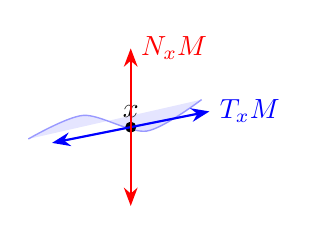
\begin{tikzpicture}[scale=1.0]
  \draw[manifold] plot[smooth] coordinates {(-1,0) (-0.3,0.3) (0.5,0.1) (1.2,0.5)};
  \fill (0.3,0.15) circle (2pt) node[above] {$x$};
  \draw[tangent] (0.3,0.15) -- ++(1,0.2) node[right] {$T_x M$};
  \draw[tangent] (0.3,0.15) -- ++(-1,-0.2);
  \draw[normal] (0.3,0.15) -- ++(0,1) node[right] {$N_x M$};
  \draw[normal] (0.3,0.15) -- ++(0,-1);
\end{tikzpicture}
\caption{Tangent--normal decomposition at a point on a manifold.}
\end{figure}

\medskip
\noindent The single most important geometric fact for generative modelling is
this: \emph{explanation is tangent; hallucination is normal.} A
generative system that attempts to explain directions in $N_x M$ is
constructing structure where none exists; meaningful predictive dynamics
must remain tangent to the data manifold.

\subsection{Admissibility-Induced Geometry}

The semantic manifold is not treated here as ontologically primitive.
Positing $M \subset \mathbb{R}^n$ as a given object would invite the
objection that lawful structure has been assumed rather than derived,
leaving the framework circular with respect to the very notion of
admissibility it is meant to ground. A stronger position, consistent
with the entropic and relational perspectives developed later in this
paper, is that manifold structure is \emph{emergent}: it arises from
compatibility, conservation, and coherence constraints on allowable
transformations rather than preceding them.

Let $\mathcal{H}$ denote the space of possible semantic histories and
let $\mathcal{A} \subset \mathcal{H}$ be the subset satisfying
three constraints simultaneously: compatibility of successive states
under the governing dynamics, conservation of invariant quantities
under transport, and sheaf coherence across overlapping contextual
regions. The semantic manifold is then defined as the maximal
connected admissible subset:
\[
M := \mathrm{Conn}(\mathcal{A}).
\]
Geometry therefore arises secondarily from persistent compatibility
relations rather than preceding them. Tangent directions are those
along which admissible deformation is possible; normal directions are
those blocked by constraint violation. The distinction between
$T_x M$ and $N_x M$ is not imposed from outside but is read off
from the structure of $\mathcal{A}$ at each point.

This constructive account resolves the circularity concern. When the
paper later asserts that coherent systems must remain tangent to the
semantic manifold, it is asserting that they must remain within the
space of admissible transformations as determined by compatibility,
conservation, and coherence---not that they must conform to an
arbitrarily specified submanifold. Hallucination, on this account,
is not merely off-manifold motion; it is inadmissible transformation:
a step that violates the constraints from which the manifold geometry
was derived in the first place.

\subsection{Intrinsic and Extrinsic Semantic Geometry}

A crucial distinction must be maintained throughout what follows
between intrinsic and extrinsic structure. Intrinsic geometry
concerns relations measurable entirely within the manifold itself:
geodesic distance, sectional curvature, topological invariants, and
the internal organization of admissible semantic trajectories.
Extrinsic geometry concerns the manner in which the manifold is
embedded into a higher-dimensional ambient representational space.
These two levels of geometric description are logically independent,
and conflating them is a source of persistent confusion in both the
technical and philosophical parts of the paper.

Let $i : M \hookrightarrow \mathbb{R}^n$ be an embedding. The
induced metric on $M$ is
\[
g_{ij} = \left\langle \partial_i i,\, \partial_j i \right\rangle,
\]
which defines the intrinsic geometry of $M$ independently of the
surrounding ambient space. By contrast, the second fundamental form
\[
\mathrm{II}(X,Y) = (\nabla_X Y)^\perp
\]
captures how the manifold bends extrinsically within $\mathbb{R}^n$.
The intrinsic Riemann curvature depends only on $g$; the extrinsic
shape operator depends on how $i$ maps $M$ into the ambient space
and can change entirely when $i$ is replaced by a different embedding
of the same intrinsic manifold.

This distinction becomes especially important in semantic and
institutional systems. A social or linguistic structure may possess
internally coherent intrinsic organization while appearing
contradictory under a compressed representational embedding that
destroys essential degrees of freedom. Bureaucratic codifications,
legal formalisms, statistical proxies, and symbolic interfaces often
induce extrinsic distortions that project intrinsically coherent
trajectories into apparently inconsistent ambient coordinates. Many
semantic pathologies are therefore embedding failures---failures of
the projection $i$---rather than failures of the underlying manifold
$M$. Repairing such pathologies does not require changing the
manifold but changing how it is represented.

Generative systems encounter the same duality. A model may remain
locally tangent to an incorrectly estimated or poorly chosen embedding
while still systematically misrepresenting the intrinsic structure of
the semantic manifold. Coherence therefore requires not only tangent
alignment in the ambient sense but sufficiently faithful embedding
geometry: the embedding must preserve the intrinsic curvature,
topology, and separation structure of $M$ well enough that
tangent-aligned dynamics in the ambient representation correspond to
admissible dynamics in the intrinsic geometry. This is why two
models can satisfy the same pointwise normal-projection condition
while differing dramatically in their semantic fidelity: one may be
working in an embedding that preserves intrinsic structure, while
the other is navigating a distorted image of the manifold.

% ============================================================
% SECTION 3 — GENERATIVE MODELS RESTRICTED TO MANIFOLDS
% ============================================================

\section{Generative Models Restricted to Manifolds}

A generative model is typically a map $G : Z \to \mathbb{R}^n$ where
$Z$ is a latent space. Under the manifold hypothesis, the image of $G$
should lie in a $d$-dimensional manifold: $G(Z) \subseteq M \subset
\mathbb{R}^n$.

\subsection{Energy formulation}

Given an observation $o \in \mathbb{R}^n$, inference seeks a latent code
$z^\ast$ minimizing an energy functional:
\[
z^\ast = \arg\min_z \mathcal{E}(z; o),
\]
where
\[
\mathcal{E}(z; o) = \|o - f(G(z))\|^2_\Sigma + \lambda \mathcal{C}(G(z)).
\]
The coherence term $\mathcal{C}$ penalizes deviations from semantic
consistency across contexts and across manifold charts. If the manifold
is equipped with an embedding $i : M \hookrightarrow \mathbb{R}^n$, then
the condition $\mathrm{dist}(G(z), M) = 0$ must be enforced.

\subsection{Tangent restriction and geometric correctness}

A generative update $\Delta x \in \mathbb{R}^n$ at state $x \in M$ must
satisfy $\Delta x \in T_x M$, or equivalently,
$\mathrm{Proj}_{N_x M} (\Delta x) = 0$.
This is the formal geometric criterion for non-hallucinatory generation.

\begin{figure}[H]
\centering
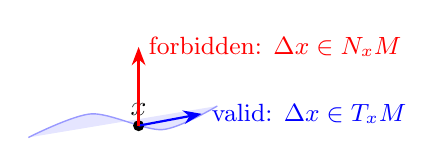
\begin{tikzpicture}[scale=1.0]
  \draw[manifold] plot[smooth] coordinates {(-1,0) (-0.2,0.3) (0.7,0.1) (1.4,0.4)};
  \fill (0.4,0.15) circle (2pt) node[above] {$x$};
  \draw[tangent] (0.4,0.15) -- ++(0.8,0.15)
    node[right] {\small valid: $\Delta x \in T_xM$};
  \draw[normal] (0.4,0.15) -- ++(0,1.0)
    node[right] {\small forbidden: $\Delta x \in N_xM$};
\end{tikzpicture}
\caption{Generative updates must remain in the tangent space.}
\end{figure}

\subsection{Why off-manifold prediction fails}

Let $x \in M$ be a semantic state. Noise $\eta \in N_x M$ has no
law-governed structure: $\eta \sim \mathcal{N}(0,\sigma^2 I_{n-d})$.
A model that attempts to represent or predict $\eta$ is mapping a
structureless distribution into a structured generator, which forces the
generator to create non-existent geometry.

\begin{theorem}[Off-Manifold Catastrophe]
Let $M$ be a $d$-manifold. Any $C^1$ generator $G$ that learns a
mapping with nonzero normal component on a set of positive measure will
produce outputs whose support has Hausdorff dimension $> d$.
\end{theorem}

\begin{proof}
$G$ maps latent space vectors to ambient space. If the Jacobian $DG$
has nonzero projection onto $N_x M$ over a non-negligible set, its
image contains an open set in directions transverse to $M$, increasing
local dimensionality, which contradicts the manifold restriction.
\end{proof}

This formalizes hallucination as a dimensionality explosion.

\subsection{Curvature Accumulation and Long-Horizon Hallucination}

Hallucination does not arise exclusively through immediate motion in
normal directions. A second and subtler failure mode occurs when a
trajectory remains locally tangent at every step while accumulating
curvature error over long temporal horizons. In such cases each
individual update appears semantically admissible, yet the integrated
trajectory diverges globally from the manifold region supporting
coherent interpretation. This phenomenon is especially important for
autoregressive systems, which generate outputs by iterating a local
prediction rule many times over, and for institutional systems, which
evolve through successive locally-approved decisions that collectively
drift far from the manifold of operational reality.

The analysis uses geodesic deviation. Let $\gamma_1(t)$ and
$\gamma_2(t)$ be nearby semantic trajectories initially close at
$t = 0$, with separation vector field $\xi^\mu$ measuring their
relative displacement. The covariant acceleration of this separation
satisfies the Jacobi equation:
\[
\frac{D^2 \xi^\mu}{dt^2}
=
R^\mu_{\ \nu\rho\sigma}\,
u^\nu u^\rho \xi^\sigma,
\]
where $R^\mu_{\ \nu\rho\sigma}$ is the Riemann curvature tensor of
$M$ and $u^\mu = \dot{\gamma}^\mu$ is the tangent velocity field.
In regions of positive sectional curvature the right-hand side acts
as a restoring force, pulling nearby trajectories toward one another.
In regions of negative sectional curvature it acts as a diverging
force, exponentially amplifying initial separations. High negative
curvature in a semantic manifold therefore makes long-horizon
coherence intrinsically difficult: even a generative system that
maintains perfect local tangent alignment at every step will produce
trajectories that diverge exponentially in the global semantic space.

This explains the characteristic failure pattern of deep autoregressive
generation: outputs remain locally fluent and semantically plausible
for many steps before undergoing sudden, large-scale semantic
collapse. The instability is not introduced by any single off-manifold
step but by exponential growth of curvature-sensitive perturbations
accumulated across many locally admissible steps. The distinction
between local tangent correctness and global geodesic stability is
therefore essential: a coherent intelligence must not only avoid
direct motion into $N_x M$ but must also regulate the curvature
environment through which its trajectories pass, ensuring that
the semantic manifold's local geometry does not amplify inevitable
small perturbations into globally incoherent outcomes. This connects
directly to the Ricci-flow regularization introduced in the semantic
phase transitions section as a mechanism for smoothing curvature
concentration and extending the domain of geodesic stability.

% ============================================================
% SECTION 4 — JIT GEOMETRIC REINTERPRETATION
% ============================================================

\section{Geometric Reinterpretation of JiT}

The ``Back to Basics'' result of Li and He~\cite{li2025backtobasics}
demonstrates that models predicting \emph{clean} data directly
outperform those predicting noised quantities even when both use
identical Transformer architectures. This section provides a geometric
explanation of that finding, drawing on the classical manifold
assumption that natural images lie on a low-dimensional, highly curved,
and locally smooth manifold $M \subset \mathbb{R}^n$, while noised
images are generically off-manifold, occupying regions with no semantic
or geometric structure.

\subsection{Clean prediction enforces tangent alignment}

Let $x \in M$ be a natural datum. A noisy version is
\[
x_t = \sqrt{\alpha_t}\, x + \sqrt{1 - \alpha_t}\,\epsilon,
\qquad \epsilon \in N_x M.
\]
Diffusion models predict $\epsilon$ or $x_t$; JiT predicts $x$.
Predicting $\epsilon$ requires representing variation in $N_x M$, which
has no structure and cannot be captured by a finite-capacity model in
high dimensions: the model must hallucinate. Predicting $x$ enforces
$G(z_t) \in M$ and $G(z_t) \approx x$, so all updates remain tangent
to $M$.

From a geometric viewpoint, predicting noise corresponds to training a
vector field $f_\theta : \mathbb{R}^n \to \mathbb{R}^n$ with
substantial support in $N_x M$, the normal bundle of the data manifold.
Such a model is inherently unstable: infinitesimal misalignment between
tangent directions and noise directions leads to divergent trajectories,
off-manifold drift, and the catastrophic generation failures observed in
high-dimensional settings~\cite{li2025backtobasics}.

When the network is instead trained to predict clean images, its learned
vector field is forced to lie within the tangent bundle $TM$. The
prediction objective enforces
\[
\mathrm{Proj}_{N_x M}\!\big(f_\theta(x)\big) \approx 0,
\]
since any component in the noise-normal direction would move the
prediction away from the ground-truth manifold. Thus, despite the
apparent weakness or under-capacity of the model, its dynamics remain
confined to an intrinsically low-dimensional space where learning is
dramatically easier.

\subsection{Transformer patching as implicit charting}

Large-patch Transformers induce local coordinate systems, effectively
learning charts $\phi_i : U_i \subset M \to \mathbb{R}^d$. The JiT
model stitches these charts via self-attention, which enforces a
sheaf-like coherence $\phi_i(x) = \phi_j(x)$ on overlaps. JiT is
therefore not merely ``just attention''---it is an implementation of a
manifold atlas.

Viewed through the lens of the CLIO framework introduced below, JiT
may be interpreted as performing a discretized gradient descent on a
learned potential defined along the data manifold. Each generative step
\[
x_{t-1} = x_t - \eta\,\nabla V_\theta(x_t)
\]
remains approximately tangent to $M$ due to the clean-data objective,
effectively implementing a Morse-like flow that contracts trajectories
toward semantically consistent regions. This is why a Transformer with
surprisingly few parameters, when trained under a clean-prediction
objective, behaves as a competent generative model: its update rule is
geometrically constrained even if its architecture is not.

\begin{theorem}[JiT = Tangent Flow Approximation]
Transformer layers in JiT implement an approximate tangent-flow update:
\[
x_{t+1} = x_t - \eta\,\Pi_{T_{x_t} M} \nabla \mathcal{L}(x_t),
\]
where $\Pi_{T_{x_t} M}$ is the orthogonal projector to the tangent space.
\end{theorem}

\begin{proof}[Sketch]
The clean-data objective forces residuals to lie in the range of
$DG(z)$, which spans $T_x M$. Thus gradient backpropagation
automatically enforces tangent projection.
\end{proof}

JiT succeeds because it accidentally obeys MAGI.

% ============================================================
% SECTION 5 — ACTIVE INFERENCE AS GEODESIC CONTROL
% ============================================================

\section{Active Inference as Geodesic Control}

Under the free-energy principle~\cite{friston2010freeenergy}, systems
minimize
\[
F[q] = \mathbb{E}_q[\log q - \log p(o,z)].
\]
If $z$ parameterizes a manifold $M$ and $G(z)$ is its embedding, the
pullback metric is
\[
g_{ij}(z) = \left\langle
\frac{\partial G}{\partial z_i},
\frac{\partial G}{\partial z_j}
\right\rangle.
\]
Gradient descent on $F$ with respect to the Riemannian structure yields
\[
\dot{z}^i = - g^{ij}(z)\, \frac{\partial F}{\partial z^j},
\]
which is a geodesic-like evolution on $M$.

\begin{figure}[H]
\centering
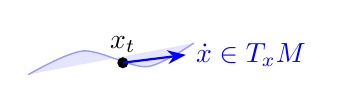
\begin{tikzpicture}[scale=1.0]
  \draw[manifold] plot[smooth] coordinates {(-1,0) (-0.3,0.3) (0.5,0.1) (1.1,0.4)};
  \fill (0.2,0.15) circle (2pt) node[above] {$x_t$};
  \draw[vector,blue] (0.2,0.15) -- ++(0.8,0.1)
    node[right] {$\dot{x} \in T_xM$};
\end{tikzpicture}
\caption{Active inference induces a Riemannian gradient flow on $M$.}
\end{figure}

Because $g_{ij} = J_i^\top J_j$ where $J = DG(z)$, the quantity
$g^{ij}\,\partial_j F$ is the natural gradient in information geometry.
Active inference is therefore, geometrically, natural gradient descent
on a manifold. Predictive coding selects directions with meaningful
semantic structure; updates are tangent projections of sensory
prediction errors; geodesic curvature encodes attentional redirection;
and all inference is constrained by the intrinsic geometry of $M$.

\subsection{Information Geometry and Semantic Distinguishability}

The manifold structure underlying MAGI is not purely geometric in the
Euclidean sense: it is informationally constrained through relations
of distinguishability. Two semantic states that cannot be distinguished
under the observational structure available to an agent are effectively
identified within the induced statistical geometry, regardless of their
coordinate distance in the ambient space. Coherent cognition therefore
depends not only on preserving tangent structure but on preserving
informationally meaningful separations between trajectories.

Let $\mathcal{P} = \{p(x|\theta) : \theta \in \Theta\}$ be a
statistical manifold parameterized by latent semantic coordinates
$\theta$. The Fisher information metric
\[
g_{ij}(\theta)
=
\mathbb{E}
\left[
\partial_i \log p(x|\theta)
\;
\partial_j \log p(x|\theta)
\right]
\]
defines the intrinsic geometry of distinguishability on $\mathcal{P}$.
Nearby semantic states with high Fisher distance are observationally
separable, while states with small Fisher distance collapse under
compression into effectively identical representations. Semantic
compression is possible at all precisely because many ambient degrees
of freedom contribute negligibly to the Fisher metric: a projection
$\pi : X \to M$ may discard large numbers of ambient dimensions while
preserving semantic coherence so long as the discarded directions
carry negligible informational curvature.

Compression becomes pathological only when the projection destroys
directions that carry significant Fisher-metric distinguishability.
Generative hallucination may therefore be interpreted as a failure of
distinguishability preservation: the model constructs trajectories
that appear locally plausible under low-order statistical tests while
violating higher-order informational invariants encoded in the
manifold geometry. This reframes the intelligence criterion once
more. A coherent intelligence is not one that models every possible
variation in ambient space but one that correctly identifies which
distinctions correspond to lawful manifold structure---large Fisher
distance---and which correspond merely to observational noise---small
or zero Fisher distance. The natural gradient $g^{ij}\partial_j F$
introduced in the active inference analysis is the computational
instantiation of this principle: it rescales gradient steps by the
Fisher metric so that the optimization dynamics respect the
informational geometry of the statistical manifold rather than its
Euclidean ambient coordinates.

% ============================================================
% SECTION 6 — SPARSE SEMANTIC PROJECTION
% ============================================================

\section{Sparse Semantic Projection}

Real perceptual data $x \in \mathbb{R}^n$ are overwhelmingly redundant.
The semantic degrees of freedom are far fewer than the ambient
dimension. Sparse semantic projection extracts the coordinates that lie
along meaningful directions---those tangent to the manifold $M$.

\subsection{Sparse semantic encoder}

Let $W$ be a learned linear operator:
\[
s = W x, \qquad s \in \mathbb{R}^k, \quad k \ll n,
\]
with a sparsity constraint $\|W\|_0 \le k$, or its $\ell_1$-regularized
convex proxy. The sparse code $s$ must correspond to a point on the
manifold, $G(s) \in M$, so the semantic projection is the composition
\[
x \xmapsto{\;W\;} s \xmapsto{\;G\;} \hat{x} \in M.
\]

\begin{definition}[Semantic Projection Operator]
A map $\Pi_{\mathrm{sem}} : \mathbb{R}^n \to M$ given by
$\Pi_{\mathrm{sem}}(x) = G(Wx)$ such that $G(Wx)$ minimizes distance
to the manifold and maximizes semantic coherence.
\end{definition}

\begin{figure}[H]
\centering
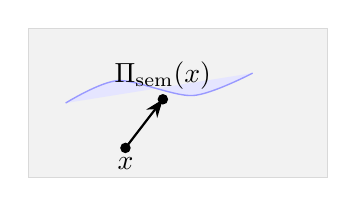
\begin{tikzpicture}[scale=0.95]
  \draw[gray!30,fill=gray!10] (-1,-1) rectangle (3,1);
  \draw[manifold] plot[smooth] coordinates {(-0.5,0) (0.2,0.3) (1.2,0.1) (2.0,0.4)};
  \fill (0.3,-0.6) circle (2pt) node[below] {$x$};
  \draw[vector] (0.3,-0.6) -- (0.8,0.05);
  \fill (0.8,0.05) circle (2pt) node[above] {$\Pi_{\mathrm{sem}}(x)$};
\end{tikzpicture}
\caption{Sparse semantic projection maps $x$ to its closest semantically meaningful point on $M$.}
\end{figure}

\subsection{Theoretical justification}

Let $M$ be a smooth manifold of reach $\tau > 0$
(Federer~\cite{federer-reach}). For any $x$ within distance $<\tau$ of
$M$, there exists a unique nearest point $\Pi(x) \in M$.

\begin{theorem}[Consistency of Sparse Projection]
If $W$ is trained to minimize reconstruction error under a manifold
regularization penalty, then $\|G(Wx) - \Pi(x)\| \le \epsilon$
for all $x$ in a sufficiently small tubular neighborhood of $M$.
\end{theorem}

\begin{proof}[Sketch]
$G(Wx)$ lies in the image of $G$, which approximates $M$; minimizing
reconstruction error forces convergence toward the nearest-point
projection.
\end{proof}

Sparse projection reduces noise, enforces manifold alignment, and
establishes a coordinate system for CLIO.

% ============================================================
% SECTION 7 — CONTEXTUAL SHEAF COHERENCE
% ============================================================

\section{Contextual Sheaf Coherence}

Perception and cognition are distributed across overlapping contexts:
visual, linguistic, proprioceptive, semantic, temporal, and so on. Each
context provides partial information about the underlying semantic
state. Sheaf theory provides the mathematical machinery to formalize how
local contexts combine into a globally consistent semantic state.

\subsection{Presheaves and the sheaf condition}

Let $\mathcal{C}$ be a category of contexts, with objects $U,V,\ldots$
representing perceptual modalities or spatial/temporal regions and
arrows $V \to U$ representing restriction relations. A presheaf assigns
semantic states $S(U)$ on context $U$ together with restriction maps
$\rho_{UV} : S(U) \to S(V)$.

\begin{definition}[Semantic Sheaf]
The semantic sheaf is a functor $S: \mathcal{C}^{op} \to \mathrm{Set}$
satisfying the sheaf axioms: if sections agree on all overlaps they
agree globally (locality), and compatible local sections can be
uniquely glued to form a global section (gluing).
\end{definition}

\begin{figure}[H]
\centering
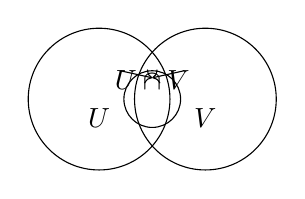
\begin{tikzpicture}[scale=0.9]
  \draw (0,0) circle (1) node[below] {$U$};
  \draw (1.5,0) circle (1) node[below] {$V$};
  \draw (0.75,0) circle (0.4) node[above] {$U \cap V$};
  \draw[->] (0.3,0.4) -- (0.75,0.3);
  \draw[->] (1.2,0.4) -- (0.75,0.3);
\end{tikzpicture}
\caption{Sheaf coherence: sections on $U$ and $V$ must agree on $U \cap V$.}
\end{figure}

\subsection{CLIO as a sheaf morphism}

Let $C : S \to S$ be a CLIO functor representing one cognitive loop
iteration.

\begin{theorem}[CLIO Coherence]
If $S$ is a sheaf and $C$ preserves restriction maps, then $C$ is a
sheaf morphism: $\rho_{UV}(C(s_U)) = C(\rho_{UV}(s_U))$.
\end{theorem}

\begin{proof}
Functoriality ensures commutation with morphisms; restriction maps are
morphisms in $\mathcal{C}^{op}$.
\end{proof}

Thus CLIO updates are guaranteed never to break contextual consistency:
cognition respects semantic gluing.

\subsection{Obstructions and Čech cohomology}

Not all compatible local sections glue globally; obstructions are
measured by the first Čech cohomology group.

\begin{definition}[Semantic Obstruction]
The obstruction to global semantic coherence across contexts is
$\mathcal{O} \in H^1(\mathcal{C}; S)$.
\end{definition}

Inconsistencies---including hallucinations---correspond precisely to the
case $\mathcal{O} \neq 0$. Failure to glue is hallucination.

\subsection{Stratification Boundaries and Semantic Crisis}

Real semantic systems are rarely globally smooth. They are typically
composed of overlapping strata with distinct local dimensionalities,
coordinate systems, and admissibility conditions. Within each stratum
$S_\alpha$ of a Whitney stratification $X = \bigsqcup_\alpha S_\alpha$,
local tangent structure is smooth and admissible semantic motion is
well-defined. At stratum boundaries, however, the effective tangent
dimension may change discontinuously and local chart compatibility may
fail. These boundary regions are not peripheral anomalies but sites of
disproportionate semantic importance.

Scientific revolutions frequently correspond to transitions between
incompatible conceptual strata: the admissibility conditions governing
Newtonian mechanics and those governing quantum mechanics cannot be
globally glued, and the transition between them is not a smooth
deformation but a stratified bifurcation in which the lower-dimensional
stratum becomes a limiting approximation of the higher-dimensional one.
Psychological fragmentation often emerges when cognitive trajectories
become trapped near singular semantic boundaries where competing local
coordinate systems cannot be globally reconciled. Institutional crises
similarly arise when systems optimized within one semantic stratum
attempt to extend their coordinate structure into domains governed by
different invariants---when administrative categories designed for one
population are applied to another for which their presuppositions fail.

The sheaf-theoretic obstruction classes introduced earlier are
particularly significant near such boundaries. A nontrivial obstruction
$\mathcal{O} \in H^1(\mathcal{C}; S)$ indicates that local semantic
coherence cannot be extended globally across the stratified space. Near
stratum boundaries this obstruction is generically nonzero: the local
charts on either side of the boundary are defined with respect to
different tangent structures and cannot be smoothly glued. Hallucination,
fragmentation, and category collapse are therefore often singularity
phenomena associated with failed transitions between incompatible
semantic strata rather than simple off-manifold excursions within a
single smooth region. A theory of semantic coherence that attends only
to smooth interiors and ignores strata boundaries will systematically
misidentify the most consequential failure modes.

% ============================================================
% SECTION 7b — PARALLEL TRANSPORT AND SEMANTIC HOLONOMY
% ============================================================

\section{Parallel Transport and Semantic Holonomy}

The sheaf-theoretic analysis in the preceding section identifies
hallucination with the failure of local semantic sections to assemble
into a globally consistent state. That analysis is essentially
combinatorial: it asks whether compatible local data can be glued. The
present section introduces the differential-geometric complement to that
picture, which is sensitive to a subtler failure mode. A trajectory may
remain locally tangent to the semantic manifold at every step while
nevertheless accumulating global inconsistency through the curvature of
the manifold itself. This is the phenomenon of semantic holonomy, and
it is not detected by the pointwise No-Noise Prediction criterion alone.

\subsection{Levi--Civita Transport and Semantic Drift}

Let $\gamma : [0,1] \to M$ be a semantic trajectory and
$V(t) \in T_{\gamma(t)}M$ a vector field transported along it. The
Levi--Civita connection $\nabla$ on $M$ defines parallel transport as
the solution to:
\[
\nabla_{\dot{\gamma}} V = 0.
\]
A transported semantic frame that satisfies this equation at every
instant drifts neither into normal directions nor, within the tangent
bundle, into artificially rotated orientations induced by path history.
Deviation from parallel transport defines a measure of semantic drift
along the path:
\[
D_\gamma(V)
=
\int_0^1
\left\|\nabla_{\dot{\gamma}} V(t)\right\|^2 dt.
\]
A coherent inferential process minimizes $D_\gamma$, maintaining the
semantic frame in as stable an orientation as the manifold geometry
permits. Large $D_\gamma$ indicates that the inference process is
introducing artificial rotations into the transported semantic context,
producing contextual inconsistency even when no single step departs
from the manifold.

\subsection{Holonomy and Global Inconsistency}

The deepest form of this phenomenon arises for closed trajectories.
Let $\gamma : [0,1] \to M$ be a loop with $\gamma(0) = \gamma(1) = x$.
Parallel transport around $\gamma$ defines a linear map
\[
P_\gamma : T_x M \to T_x M,
\]
the holonomy operator of the loop. When $M$ is flat, $P_\gamma$ is the
identity: transport around any closed loop returns the frame to its
original orientation. When $M$ is curved, $P_\gamma \neq \mathrm{id}$
in general, and the discrepancy
\[
\mathcal{H}_\gamma(V) = P_\gamma(V) - V
\]
represents the holonomy accumulated by transport around the loop.
In the semantic context this has a direct interpretation: a cognitive
or generative system that traverses a closed contextual loop and
returns to the same semantic state with a rotated frame has
accumulated a form of global inconsistency invisible to any local
analysis. The system's local updates were all admissible, its pointwise
normal projections were all zero, and yet the global trajectory has
introduced incompatibility between the initial and final semantic
orientations.

This distinction formalizes two qualitatively different failure modes
that the paper's earlier sections were conflating. Local hallucination
is instantaneous normal-direction drift: $\mathrm{Proj}_{N_x M}(f(x))
\neq 0$ at a single point. Transport inconsistency is accumulated
holonomy: the frame returned to a point after traversal of a closed
loop is rotated relative to the frame that departed. Many
institutional, linguistic, and cognitive failures belong to the second
category rather than the first. Individual inferential steps remain
plausible in isolation while the cumulative trajectory drifts into
global incoherence through curvature effects. This is why fragmented
media environments and recursive institutional policy cycles can
generate internally consistent local narratives that are mutually
incompatible globally: they are traversing different closed loops on a
curved semantic manifold and accumulating distinct holonomies.

The sheaf obstruction class $\mathcal{O} \in H^1(\mathcal{C}; S)$
and the holonomy group of $M$ are therefore complementary diagnostics.
The former detects discrete gluing failure across contextual patches;
the latter detects continuous orientation drift under transport around
smooth paths. A fully coherent system requires both to vanish.

% ============================================================
% SECTION 8 — RSVP FIELDS AS SEMANTIC GEOMETRY
% ============================================================

\section{RSVP Fields as Semantic Geometry}

The RSVP (Relativistic Scalar Vector Plenum) framework models semantic
dynamics in terms of three fields: an entropy field $\Phi$, a vector
flow $\mathbf{v}$, and a semantic potential $S$. We reinterpret these
fields geometrically.

A semantic manifold arises as a sublevel set of $\Phi$:
$M = \{ x \in \mathbb{R}^n \mid \Phi(x) = \Phi_0 \}$.
Entropy gradients determine allowable semantic transitions, with high
curvature in $\Phi$ indicating regions where semantic complexity is
high or transitions are unstable. The vector field $\mathbf{v}$ defines
directional flow across the manifold, $\dot{x} = \mathbf{v}(x)$, and
semantically meaningful dynamics must preserve manifold structure:
$\mathbf{v}(x) \in T_x M$. RSVP vector flow thus enforces
tangent-constrained transport.

The semantic landscape has critical points corresponding to attractors,
stable interpretations, and choices; $S$ is naturally interpreted as a
Morse function on $M$, with critical points of $S$ corresponding to
stable semantic states.

\begin{theorem}[RSVP--Morse Correspondence]
If $S$ is generically perturbed, it is a Morse function whose gradient
flow preserves the manifold structure: $-\nabla S(x) \in T_x M$.
\end{theorem}

\begin{proof}
Generic perturbation yields a Morse function by Sard--Smale. Since $S$
is defined intrinsically on $M$, its gradient is tangent.
\end{proof}

\begin{figure}[H]
\centering
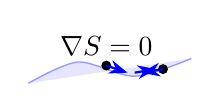
\begin{tikzpicture}[scale=0.9]
  \draw[manifold] plot[smooth] coordinates {(-1,0) (-0.3,0.3) (0.5,0.1) (1.3,0.35)};
  \fill (0.1,0.25) circle (2pt) node[above] {$\nabla S = 0$};
  \fill (0.9,0.2) circle (2pt);
  \draw[vector,blue] (0.1,0.25) -- ++(0.3,-0.1);
  \draw[vector,blue] (0.5,0.15) -- ++(0.3,0.05);
  \draw[vector,blue] (0.9,0.2) -- ++(-0.3,-0.05);
\end{tikzpicture}
\caption{Semantic manifold with Morse potential and tangent-constrained RSVP flow.}
\end{figure}

RSVP thus becomes a field-theoretic version of manifold semantic
dynamics, providing the continuous substrate on which MAGI operates.

% ============================================================
% SECTION 8b — SEMANTIC PHASE TRANSITIONS AND SINGULARITY FORMATION
% ============================================================

\section{Semantic Phase Transitions and Singularity Formation}

Morse theory, as developed in Sections~9 and~A.4, describes the smooth
critical structure of the semantic potential landscape: isolated
nondegenerate critical points, stable and unstable manifolds, gradient
flows that converge to well-defined attractors. This picture is
adequate for systems that evolve slowly through a stable manifold
geometry. Real cognitive, institutional, and generative systems,
however, are subject to conditions under which the manifold itself
changes topology---where the ambient curvature accumulates faster than
the system can adapt and where the smooth landscape undergoes abrupt
bifurcation. These events are not smooth critical transitions in the
Morse sense; they are semantic phase transitions, topological changes
in $M$ itself that the framework must be able to characterize.

Let $M_t$ be a time-dependent semantic manifold with metric $g(t)$.
The curvature of $M_t$, measured by the Riemann tensor $Rm(x,t)$,
may accumulate in local regions under sufficiently rapid semantic
compression or contradictory update pressure. A singularity forms
when:
\[
\sup_{x \in M_t} |Rm(x,t)| \to \infty.
\]
At the singularity, the local coordinate system ceases to be coherent:
tangent spaces become ambiguous or discontinuous, the
tangent-normal decomposition that grounds the No-Noise Prediction
Theorem loses its well-definedness, and the smooth Morse flow
structure breaks down. These regions correspond geometrically to
conceptual bifurcation, where a semantic attractor basin splits
into two or more incompatible basins; to category collapse, where
the manifold dimension drops and previously distinct semantic
directions become identified; or to semantic fracture, where the
manifold loses connectivity and previously reachable regions
become inaccessible.

In the context of generative models, singularity formation explains
why certain failure modes are not merely quantitatively severe but
qualitatively discontinuous: the system does not gradually worsen
but suddenly loses access to coherent generation in an entire
semantic region. In the civilizational analysis of Section~19,
singularity formation provides the geometric correlate of
institutional collapse: not simply large-scale off-manifold drift
but a topological bifurcation of the proxy manifold into components
that can no longer be reconnected by any admissible trajectory.
In cognition, it corresponds to the abrupt dissolution of a
conceptual framework under conditions that cannot be accommodated
by smooth belief revision.

Ricci flow provides one natural mechanism for studying and
potentially preventing singularity formation. The flow
\[
\partial_t g_{ij} = -2 R_{ij}
\]
evolves the metric in the direction of decreasing curvature,
smoothing out curvature concentration and delaying or preventing
singularity formation in regions that can be reached by the flow.
Applied to the semantic manifold, Ricci-flow-inspired regularization
would smooth the metric structure of the potential landscape,
distributing curvature more uniformly and reducing the risk of
local singularity formation under rapid update pressure. This
connects the framework to Perelman's surgery techniques for
handling unavoidable singularities: in regions where curvature
concentration cannot be prevented, controlled topological surgery
replaces the singular region with a lower-curvature substitute,
allowing the flow to continue beyond the singularity. The semantic
analogue would be a controlled conceptual restructuring that
replaces a fractured semantic region with a coherent lower-complexity
representation, preserving global manifold connectivity at the cost
of local dimensional reduction.

% ============================================================
% SECTION 9 — CLIO FUNCTORS AS MORSE FLOWS
% ============================================================

\section{CLIO Functors as Morse Flows}

CLIO (Cognitive Loop via In-Situ Optimization) models cognition as a
recursive loop: perception feeds a model, the model generates
predictions, predictions drive action, action returns to perception.
Each CLIO iteration is a step of negative gradient flow on a Morse
potential $S$ defined on the manifold $M$.

\subsection{Cognitive loop operators as functors}

Let $\mathbf{Sem}$ be the category of semantic states with morphisms
representing structure-preserving semantic transformations. A CLIO
update is a functor $C : \mathbf{Sem} \to \mathbf{Sem}$.

\begin{definition}[CLIO Functor]
A functor $C$ is a CLIO functor if it satisfies three conditions:
stability (fixed points corresponding to semantic equilibria),
monotonicity (each update reduces semantic free energy), and naturality
(for any semantic morphism $f$, $C \circ f = f \circ C$).
\end{definition}

These conditions mirror the requirements for Morse flows.

\subsection{Constructing the Morse potential}

Let $L$ denote the total semantic loss functional (prediction error
plus coherence penalty). We define the Morse potential
\[
S(x) = L(x) + \epsilon R(x),
\]
where $R$ is a generic perturbation and $\epsilon > 0$ ensures $S$ is
Morse by the Sard--Smale theorem. A CLIO iteration then takes the form
\[
x_{t+1} = x_t - \eta\,\nabla_M S(x_t),
\]
where $\nabla_M$ is the Riemannian gradient on the manifold.

\begin{theorem}[CLIO--Morse Equivalence]
Every CLIO functor $C$ corresponds locally to a single gradient step
of a Morse function $S$:
\[
C(x) = \mathrm{Exp}_x \big(-\eta \nabla_M S(x)\big),
\]
and conversely, every Morse function generates a CLIO functor.
\end{theorem}

\begin{proof}
Naturality ensures $C$ preserves manifold structure. Monotonicity
implies existence of a Lyapunov function $S$. Stability yields critical
points. Morse structure follows from generic perturbation. The
exponential map expresses local flow.
\end{proof}

\begin{figure}[H]
\centering
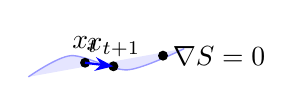
\begin{tikzpicture}[scale=0.9]
  \draw[manifold] plot[smooth] coordinates {(-1,0) (-0.4,0.3) (0.4,0.1) (1.2,0.4)};
  \fill (-0.2,0.2) circle (2pt) node[above] {$x_t$};
  \fill (0.2,0.15) circle (2pt) node[above] {$x_{t+1}$};
  \draw[vector,blue] (-0.2,0.2) -- (0.2,0.15);
  \fill (0.9,0.3) circle (2pt) node[right] {$\nabla S = 0$};
\end{tikzpicture}
\caption{One CLIO iteration corresponds to a step along $-\nabla S$ on $M$.}
\end{figure}

Cognition is Morse theory on a semantic manifold.

% ============================================================
% SECTION 10 — THE MASTER FUNCTIONAL
% ============================================================

\section{The Master Functional}

We now unify free energy, sparsity, sheaf coherence, manifold
alignment, and RSVP fields into a single variational principle. Let
$\mathcal{J}[s, W, G, S, \Phi, \mathbf{v}]$ be the total
generative--semantic--cognitive functional:
\begin{align}
\mathcal{J}
= &\underbrace{F[q(s)]}_{\text{free energy}}
+ \lambda_1 \underbrace{\|W\|_1}_{\text{sparsity}} \notag \\
&+ \lambda_2 \underbrace{\sum_{U,V} \|s_U - \rho_{VU}(s_V)\|^2}_{\text{sheaf coherence}} \notag \\
&+ \lambda_3 \underbrace{\mathrm{dist}^2(G(s), M)}_{\text{manifold constraint}} \notag \\
&+ \lambda_4 \underbrace{\int_M \left(\|\nabla \Phi\|^2 + \|\mathbf{v}\|^2 + \|S\|^2\right) d\mu}_{\text{RSVP field energy}}.
\end{align}

\subsection{Optimality conditions}

Minimizing $\mathcal{J}$ yields a sparse semantic encoder $W^\ast$, a
manifold-aligned latent state $s^\ast$, an embedding $G^\ast$ that
parameterizes $M$, a Morse potential $S^\ast$ giving stable semantic
equilibria, and RSVP entropy and flow fields $\Phi^\ast,\,\mathbf{v}^\ast$.

\begin{theorem}[Unified Euler--Lagrange System]
Critical points of $\mathcal{J}$ satisfy a coupled system of
Euler--Lagrange equations linking
\[
\delta_s \mathcal{J} = 0, \quad
\delta_W \mathcal{J} = 0, \quad
\delta_G \mathcal{J} = 0, \quad
\delta_S \mathcal{J} = 0, \quad
\delta_{\Phi,\mathbf{v}} \mathcal{J} = 0.
\]
\end{theorem}

Complete proofs are provided in Appendix~D.

\subsection{Semantic Conservation Laws}

The variational structure of the master functional implies the
existence of conserved semantic quantities wherever the dynamics
preserve a symmetry of the manifold. This introduces a Noether-like
interpretation of semantic coherence that deepens the physics analogy
while remaining formally grounded.

Suppose there exists a one-parameter family of transformations
$\phi_t : M \to M$ preserving the master functional,
$\mathcal{J}[\phi_t(x)] = \mathcal{J}[x]$, with infinitesimal
generator $\mathbf{v}$. The condition that $\phi_t$ preserves the
metric structure of $M$ is expressed by the vanishing Lie derivative:
\[
\mathcal{L}_{\mathbf{v}}\, g = 0,
\]
meaning $\mathbf{v}$ is a Killing field for the Riemannian structure
induced on $M$. By the variational analogue of Noether's theorem,
such a symmetry generates a conserved quantity along the flow: a
scalar invariant that is preserved by all trajectories respecting the
symmetry and destroyed by those that do not.

In the semantic context, conserved quantities under such symmetries
correspond to stable conceptual identities. In cognition, an invariant
preserved across changes in sensory modality, context, or representational
format corresponds to an abstract concept that the system has genuinely
learned rather than memorized in a context-specific coordinate. In
institutions, invariants preserved across changes in personnel, notation,
or administrative structure correspond to organizational knowledge
that survives individual turnover. In scientific paradigms, invariants
preserved across changes in notation or formalism correspond to the
genuinely explanatory content of a theory, as opposed to its
contingent coordinate representation. In language, relational semantic
invariants maintained despite surface-level symbolic transformation
correspond to the meanings that translation preserves.

This perspective deepens the geometric account of alignment. Coherent
systems preserve semantic invariants because their flows respect the
underlying symmetry structure of the manifold. Hallucinatory or
drifting systems destroy invariants by introducing dynamics that break
symmetry---that treat the manifold asymmetrically in ways unsupported
by the admissibility constraints that generated it. The loss of a
conservation law is therefore a geometric diagnostic of semantic
pathology, complementing the normal-projection criterion of the
No-Noise Prediction Theorem with a global dynamical condition: a
system that preserves the right invariants under the right symmetries
is coherent, regardless of what its individual update steps look like
locally.

% ============================================================
% SECTION 11 — THE NO-NOISE PREDICTION THEOREM
% ============================================================

\section{The No-Noise Prediction Theorem}

We now state the central theoretical result of the paper.

\begin{theorem}[No-Noise Prediction Theorem]
Let $M$ be the semantic manifold and $N_x M$ its normal bundle.
A generative model $G$ is semantically aligned if and only if
\[
\mathrm{Proj}_{N_{G(s)} M}(f(G(s))) = 0
\quad
\text{for all $s$.}
\]
\end{theorem}

\noindent Semantically aligned generative models never produce updates
in normal directions.

\begin{proof}
($\Rightarrow$) If $G(s) \in M$, any valid predictive update moves
within $T_x M$; otherwise $G$ would leave the semantic manifold. Thus
the prediction error must satisfy the zero normal component condition.
($\Leftarrow$) If prediction errors always have zero normal component,
then the update direction is tangent at every step, so the entire
generative trajectory remains within $M$.
\end{proof}

This theorem exactly characterizes hallucination (normal-component
prediction) and semantic coherence (tangent-only prediction).

\subsection{Tangent and Normal Noise: A Necessary Refinement}

The No-Noise Prediction Theorem as stated might be misread as
a prohibition on all stochasticity, which would be incorrect and
damaging to the framework's applicability. Biological cognition,
diffusion-based exploration, variational inference, and
optimization all require controlled variation; the claim that
noise is pathological must therefore be stated with geometric
precision rather than as a blanket ban on variance.

The refinement proceeds by decomposing any perturbation field
$\eta$ at a point $x \in M$ according to the tangent-normal
splitting:
\[
\eta = \eta_T + \eta_N,
\qquad
\eta_T \in T_x M,
\quad
\eta_N \in N_x M.
\]
The tangent component $\eta_T$ represents structured stochastic
variation along directions supported by the manifold. Such
variation is not merely tolerated but necessary: it drives
exploration of the admissible semantic space, enables
variational inference to avoid degenerate fixed points, and
corresponds in biological systems to the controlled variability
that underlies learning and adaptation. The normal component
$\eta_N$ represents variation in directions orthogonal to all
lawful structure. This component has no stable continuation
under semantic transport, contributes no persistent information
to the trajectory, and is what the No-Noise Prediction Theorem
properly prohibits.

The theorem therefore asserts $\|f_N(x)\| \to 0$, not $\|\eta_T\| \to 0$.
Tangent noise is admissible and often essential. Normal noise
is structureless perturbation that, if modelled as geometry,
produces dimensionality explosion as shown in the
Off-Manifold Catastrophe theorem. The phrase ``never predict
noise'' means precisely: never allocate predictive capacity to
directions in $N_x M$. It does not mean: eliminate uncertainty
or collapse the generative distribution to a point mass.

\subsection{The Semantic Coherence Functional}

The framework to this point characterizes alignment through a
pointwise criterion. A richer characterization tracks how
well a trajectory $\gamma : [0,1] \to M$ preserves semantic
coherence globally, integrating both geometric deviation
from manifold flow and accumulated sheaf obstruction along
the path. Define the semantic coherence functional:
\[
\mathcal{C}(\gamma)
=
\int_0^1
\left(
\|\nabla_{\dot{\gamma}}\dot{\gamma}\|^2
+
\lambda \|\mathcal{O}_\gamma(t)\|^2
\right) dt,
\]
where the first term measures geodesic deviation---how far
the trajectory accelerates away from the free geodesic of the
Riemannian structure on $M$---and the second term measures
accumulated sheaf obstruction density along $\gamma$, with
$\lambda > 0$ a weighting constant. A trajectory is
semantically coherent to the extent that $\mathcal{C}(\gamma)$
is small. Hallucination, in this functional formulation,
corresponds to $\mathcal{C}(\gamma) \to \infty$: the
trajectory either accelerates violently off the geodesic
structure of the manifold, or accumulates contextual
inconsistencies that cannot be resolved by any global
sheaf section, or both simultaneously. This functional
provides a basis for the operationally measurable coherence
metrics discussed in Appendix~D and makes the alignment
condition quantitative rather than merely qualitative.

% ============================================================
% SECTION 11b — GAUGE SYMMETRY AND SEMANTIC EQUIVALENCE
% ============================================================

\section{Gauge Symmetry and Semantic Equivalence}

The atlas structure introduced in the manifold definition of
Section~2---a collection of charts $\{(U_i, \phi_i)\}$ with smooth
transition maps on overlaps---carries a natural gauge-theoretic
interpretation that unifies the sheaf-consistency conditions of
Section~7 with the coordinate-change structure implicit throughout
the paper. Different cognitive systems, different modalities, or
different temporal contexts may represent the same semantic content
using distinct local coordinate gauges over the same underlying
manifold. The question of whether two representations encode the
same meaning is therefore the question of whether they are related
by an admissible gauge transformation.

Let $\{(U_i, \phi_i)\}$ be an atlas on $M$ with a structure group
$G$. On each overlap $U_i \cap U_j$ there is a transition function
$g_{ij} : U_i \cap U_j \to G$ relating the two charts:
\[
\phi_j = g_{ij} \circ \phi_i.
\]
Two semantic representations are gauge-equivalent if they are
related by such a smooth transition. Hallucination, in this
vocabulary, corresponds not to a coordinate change between
equivalent representations but to a failure of gauge compatibility:
the transition functions on a triple overlap fail to satisfy the
cocycle condition
\[
g_{ij} \cdot g_{jk} \cdot g_{ki} = \mathrm{id},
\]
which is precisely the condition for the local chart data to glue
into a globally consistent manifold. When the cocycle condition
fails, the atlas does not describe a coherent manifold; the local
coordinate systems are mutually inconsistent in a way that no
gauge transformation can repair.

This formulation connects three previously separate structures in
the paper. The sheaf obstruction class $\mathcal{O} \in H^1(\mathcal{C}; S)$
is the Čech-cohomological encoding of exactly this cocycle
failure: it measures the obstruction to assembling locally
gauge-consistent data into a global section. The holonomy group
computed in Section~7b measures how gauge frames rotate under
parallel transport around closed loops. And the admissibility
condition $M = \mathrm{Conn}(\mathcal{A})$ from Section~2 determines
which gauge transformations are admissible in the first place,
since only transformations that preserve compatibility,
conservation, and coherence constraints belong to the structure
group $G$.

\subsection{Semantic Fiber Structure}

The gauge-theoretic perspective also suggests a natural
algebraic structure for semantic equivalence. Let
$\Phi : \Theta \to \mathcal{F}$ be a realization map from a space
$\Theta$ of parameters or configurations to a space $\mathcal{F}$
of semantic functions. The fiber over a semantic function $f \in
\mathcal{F}$ is the set of all parameterizations that realize it:
\[
\Phi^{-1}(f) = \{\theta \in \Theta : \Phi(\theta) = f\}.
\]
This fiber collects all configurations that are semantically
equivalent under the realization map, providing a rigorous
definition of ``same meaning under different representations.''
Without this structure, semantic equivalence remains intuitive
and the framework cannot formally distinguish genuine semantic
synonymy from accidental surface similarity.

The fiber-dimension results from the theory of polynomial semantic
manifolds establish that typical fibers are positive-dimensional,
meaning that each semantic function is realized by a
positive-dimensional family of configurations. This redundancy
is not a defect but a structural feature: it corresponds to the
gauge freedom of choosing among equivalent representations,
and it is what makes the sheaf-coherence and gluing conditions
non-trivial. Two representations that lie in the same fiber are
gauge-equivalent and carry identical semantic content. Two
representations in different fibers are semantically distinct
regardless of their coordinate proximity in $\Theta$.

% ============================================================
% SECTION 12 — RELATED WORK
% ============================================================

\section{Related Work}

\paragraph{Manifold Learning.}
Foundational methods such as Isomap~\cite{tenenbaum2000isomap} and
LLE~\cite{roweis2000lle} established the algorithmic basis for
nonlinear dimensionality reduction. MAGI differs by imposing a
Whitney-stratified structure, enforcing tangent/normal decomposition
theorems, and integrating manifold learning with semantic cognition.

\paragraph{Diffusion and Score-Based Models.}
Key works~\cite{ho2020denoising,song2021scorebased,karras2022elucidating}
predict noise or score fields with substantial support in $N_x M$,
which is the fundamental flaw in MAGI terms. The JiT
paper~\cite{li2025backtobasics} demonstrates that predicting clean data
provides superior empirical performance; MAGI explains why: noise lies
in the normal bundle, while clean data lies on $M$.

\paragraph{Flow Matching.}
Works such as~\cite{lipman2023flow} learn vector fields in $\mathbb{R}^n$.
MAGI enforces $v(x) \in T_x M$, yielding flow matching with
tangent constraints.

\paragraph{Active Inference and Free Energy.}
The free-energy principle~\cite{friston2010freeenergy,parr2022}
provides the variational substrate for MAGI, here reinterpreted as
geodesic gradient flow on a Riemannian statistical manifold.

\paragraph{Geometric Deep Learning.}
Equivariant networks~\cite{bronstein2021geometric} exploit symmetry
constraints; MAGI complements this by using Morse theory, manifold
embeddings, and sheaf constraints on semantic coherence.

\paragraph{Sheaf Models.}
Recent applications to multi-modal inference~\cite{robinson2021sheaves}
provide the contextual coherence machinery; MAGI extends this with
Morse-theoretic flows, CLIO functorial updates, and stability theorems.

\paragraph{Neural ODEs.}
Neural ODEs~\cite{chen2018neuralode} learn continuous-time dynamics in
$\mathbb{R}^n$; MAGI requires $dx/dt \in T_x M$.

\medskip
\noindent Taken together, the technical literature confirms that the
core difficulty in generative modelling is not expressivity but
geometric discipline. The manifold constraint is not a
special-case assumption grafted onto standard architectures; it is
the condition that separates coherent generation from noise
amplification at every level of the existing literature. The
following sections extend this diagnosis beyond the computational
domain to show that the same failure mode---optimizing into
unsupported dimensions of an ambient space while ignoring the
intrinsic geometry of the underlying manifold---appears with equal
structural regularity in statistical reasoning about human
populations, in the logical pathologies of natural language, in
the large-scale dynamics of institutional and civilizational
systems, and finally in the design criteria for intelligence
itself. The geometry does not change when the scale changes.

% ============================================================
% SECTION 13 — SOCIAL HALLUCINATION AND STATISTICAL NORMALITY
% ============================================================

\section{Social Hallucination and Statistical Normality}

The geometric account of hallucination developed in the preceding
sections is not confined to machine learning systems. Human societies
routinely exhibit the same structural failure: the confusion of local
statistical averages with universal lawful structure, and the
subsequent misidentification of deviation from those averages as
defect rather than as variation intrinsic to the population manifold
itself.

A normal distribution does not assert moral hierarchy. It describes
a density over a space of possibilities. The mean is the most
frequently occurring point in a particular sample, not the most
correct or most valuable point in any ontological sense. Yet social
institutions persistently treat statistical centrality as prescriptive
rather than descriptive, collapsing the distributional manifold of
human variation into a narrow proxy optimized for administrative
legibility. Individuals are implicitly instructed to suppress
dimensions of themselves that do not project cleanly onto the local
average, regardless of whether those dimensions carry genuine
structural information.

This is social hallucination in a precise geometric sense. The
institution constructs an imaginary target individual who does not
exist anywhere in the actual population and then optimizes its
evaluation procedures toward that phantom. The optimization gradient
is directed into normal directions of the actual human manifold, not
tangent ones. Individuals who respond by genuinely suppressing
their admissible variation are not becoming more coherent; they are
being forced off their intrinsic trajectory.

Formally, let $\mathcal{H}$ denote the manifold of human variation,
and let $\bar{x} \in \mathcal{H}$ denote a local sample mean. The
tangent space $T_{\bar{x}} \mathcal{H}$ contains directions of
structured, lawful variation across the population. A social norm
$\mathbf{n} \in N_{\bar{x}} \mathcal{H}$ that demands convergence
toward $\bar{x}$ enforces motion in a direction orthogonal to
genuine population structure. The No-Noise Prediction Theorem
therefore applies directly: pressure to optimize toward
$\mathbf{n}$ drives a system off the manifold of coherent human
organization and into unsupported representational space.

The distribution moreover changes substantially across context.
A locally unusual feature may be near the center of an entirely
different population, professional community, or cultural manifold.
The person who appears to deviate maximally in one coordinate system
may occupy a perfectly ordinary position within the appropriate
intrinsic geometry. Restricting one's sample of human contexts too
early is therefore epistemically catastrophic: local averages
masquerade as universal truths, and the resulting social geometry
is systematically distorted by insufficient coverage of the actual
manifold.

Healthy social organization therefore requires something analogous
to the MAGI alignment condition: an institutional architecture that
preserves admissible variation rather than compressing all
trajectories toward a single attractor basin. This is not a claim
against shared norms or coordination. It is a claim that the
enforcement of excessive geometric uniformity destroys structural
information and produces exactly the kind of off-manifold drift
that the No-Noise Prediction Theorem characterizes as incoherence.
The tails of the distribution are not external to the population
manifold. They are part of it, and a society that systematically
ablates them degrades its own representational capacity.

The social case illuminates something important about what the
manifold hypothesis means outside of machine learning. In all
of the preceding sections the manifold $M$ was the object of
inference: a system tries to learn $M$ from data and succeeds
or fails depending on whether its generative dynamics remain
tangent. In the social case the manifold is not hidden. It is
constituted by the actual pattern of human variation, and
the question is whether institutional representations preserve
or destroy the structure of that pattern. The two cases share
a common failure mode---motion into normal directions---but
the social instance makes it clear that the failure is not
merely computational. It is also semantic, because the
dimensions being suppressed carry meaning that the compressed
representation cannot recover. That semantic dimension of the
failure becomes even more explicit when the source of the
off-manifold pressure is not statistical convention but the
logical structure of language itself.

% ============================================================
% SECTION 14 — CATEGORY ERRORS AND SEMANTIC PATHOLOGY
% ============================================================

\section{Category Errors and Semantic Pathology}

A parallel class of hallucination arises not from distributional
misidentification but from malformed coordinate construction. Many
apparent philosophical paradoxes, and a significant proportion of
the fluent failures produced by large language models, are not
failures of reasoning within a valid semantic space. They are
attempts to navigate regions of conceptual space that possess no
lawful manifold structure whatsoever.

Consider the classical puzzle of the unstoppable force meeting the
immovable object. The sentence is grammatically well-formed, the
constituent concepts are individually familiar, and the question
appears to invite a determinate answer. But the two predicates are
mutually exclusive by definition: a universe containing an
unstoppable force cannot contain an immovable object. The question
does not describe an underspecified problem awaiting resolution. It
describes a point in semantic space with no preimage in any
consistent world-model. Attempting to answer it by extension from
either concept is precisely the error of predicting noise: the
generator moves into normal directions because it has been given
a target that lies entirely outside the manifold of coherent
propositions.

Formally, let $\mathcal{S}$ denote the manifold of semantically
admissible propositions. A well-formed question corresponds to a
point $q \in \mathcal{S}$ from which lawful inference proceeds
along $T_q \mathcal{S}$. A category-defective question corresponds
to a specification $q \notin \mathcal{S}$, lying in the ambient
space outside the semantic manifold. Any system that produces a
fluent response to such a query is not reasoning; it is generating
a trajectory through ambient representation space in directions
entirely unsupported by the intrinsic geometry of meaning.

Natural language permits syntactic combinations that outrun
ontological admissibility. A sentence can be grammatical without
being semantically lawful, and it can be semantically locally
coherent without assembling into a globally consistent manifold
section. The sheaf condition from \S7 applies here with full
force: local coherence in each linguistic constituent does not
guarantee the existence of a global section over the full
propositional structure. Category errors are precisely cases
where the gluing condition fails, producing an obstruction
class $\mathcal{O} \in H^1(\mathcal{C}; \mathcal{S})$ that
prevents any consistent semantic assembly.

This framework clarifies why fluent hallucination is structurally
distinct from factual error. A system making a factual error
remains on the semantic manifold but arrives at the wrong point
within it; in principle the error is correctable by better
inference. A system producing fluent hallucination has departed
from the manifold entirely, generating a trajectory that is
locally smooth in ambient representation space but globally
unsupported. No amount of additional inference within the
off-manifold region recovers coherence, because coherence is a
property of the manifold, not of the trajectory within ambient
space.

This observation has direct implications for the design of
generative systems. Architectures trained to maximize predictive
continuity in ambient representation space will inevitably learn
to traverse category-defective regions fluently, because the
training objective rewards local syntactic smoothness regardless
of whether the trajectory remains on the semantic manifold. The
alignment condition $\mathrm{Proj}_{N_q \mathcal{S}}(f(G(s))) = 0$
is violated structurally by any objective that does not
explicitly penalize off-manifold generation. Category hygiene
is therefore not a post-hoc filtering problem but a constraint
that must be enforced geometrically at the level of the
generative dynamics themselves.

Both failures examined so far---the social compression of human
variation into artificially narrow norms, and the linguistic
generation of trajectories through semantically unsupported
space---are local in scope. A single institution distorts the
manifold it governs; a single language model hallucinates
within a single exchange. But the same geometric pathology
operates at a far larger scale when the system doing the
generating is not an institution or a model but a civilization.
The manifold in that case is the full ecology of physical,
biological, and social constraint within which collective
human life is embedded, and the normal directions being
optimized are correspondingly larger in consequence. The
mechanism, however, is identical.

% ============================================================
% SECTION 15 — CIVILIZATION AS A PREDICTIVE SYSTEM
% ============================================================

\section{Civilization as a Predictive System}

A civilization is a generative system at scale. It maintains
internal representations of physical reality, social structure,
human needs, and temporal continuity, and it recursively
optimizes collective behavior against those representations.
The same geometric conditions that govern coherence in individual
cognitive systems and machine learning models therefore apply,
at a different scale and with different feedback timescales, to
civilizational organization.

A healthy civilization preserves contact with the underlying
manifold of real constraints: ecological carrying capacity,
physical production, embodied human welfare, social cohesion
across time, and the long-run dynamics of the systems on which
material life depends. Its institutional representations track
variation in the tangent directions of that reality manifold,
and its optimization gradients descend toward attractor basins
that correspond to genuinely stable configurations.

Civilizational pathology, in geometric terms, is drift into
normal directions. This occurs when the institutional
representations that guide collective optimization become
decoupled from the intrinsic geometry of the underlying
reality manifold. The system continues to optimize, but the
objective landscape it navigates is a projection into
unsupported dimensions rather than a faithful image of lawful
constraint.

The specific mechanisms are by now familiar. Financial
derivatives several steps removed from material production
parameterize degrees of freedom orthogonal to any stable
economic manifold. Bureaucratic metrics substituted for
the underlying human conditions they were designed to track
become optimization targets in their own right, pulling
institutional trajectories away from the semantic manifold
of actual welfare. Engagement metrics that reward attention
capture rather than epistemic quality redirect entire
information ecosystems into high-dimensional noise. Political
signaling that is optimized for internal coalition coherence
rather than governance outcome generates trajectories
smooth in symbolic space and meaningless in policy space.
In each case the structure is identical: a proxy is
mistaken for the underlying manifold, and optimization
pressure is applied along directions orthogonal to real
constraint.

Once this drift is underway, the system's internal
representations begin to reinforce one another. Institutions
that evaluate performance using off-manifold metrics produce
incentive landscapes that reward off-manifold behavior. The
agents best adapted to the distorted landscape outcompete
those maintaining alignment with the underlying manifold.
Feedback loops consolidate the drift. The map consumes the
territory not metaphorically but through an actual geometric
mechanism: the manifold of institutional representation
diverges from the manifold of physical and social reality
until the two share no significant tangent structure.

The RSVP framework offers a natural language for this
civilizational drift. The entropy field $\Phi$ encodes
accumulated structural information about the real manifold.
As proxy optimization intensifies, $\Phi$ develops
increasingly steep gradients between the institutional
representation and the reality it purports to track.
The vector flow $\mathbf{v}$ that once transported
collective attention toward regions of lawful constraint
rotates into the normal bundle. The semantic potential $S$,
which once encoded genuine attractors of stable social
organization, is replaced by artificial critical points
generated by recursive self-referential optimization.

Recovery requires what may be called manifold re-anchoring:
the reintroduction of institutional feedback loops that
penalize normal-direction drift and reward tangent-constrained
flow with respect to the underlying reality manifold. This is
difficult precisely because the agents with the most power
to redirect the system are typically those whose position
was established by excelling at the distorted objective.
They have the least incentive to re-anchor to a manifold
that would redistribute advantage. Civilizational coherence
thus requires institutional design that structurally enforces
geometric fidelity independent of the short-run interests
of the agents currently operating within the system.

The analysis across the last three sections has moved from
the individual to the population to the civilization, and in
each case the same structure has appeared: a system that once
tracked the tangent directions of a real constraint manifold
gradually develops optimization pressure into normal
directions, generates representations that have no support
in the underlying geometry, and accumulates incoherence until
the gap between its internal model and the manifold it was
meant to track becomes irreparable without external correction.
This pattern suggests that the problem is not incidental to
any particular domain. It is a general property of systems
that optimize without explicit geometric constraints on
their representational dynamics. The question then becomes
whether it is possible to define, and eventually to
construct, systems that are constitutively incapable of
this drift---systems whose architecture encodes the manifold
constraint not as a regularizer that can be overridden by
a sufficiently strong loss signal but as a structural invariant.
That is the question taken up in the section that follows.

% ============================================================
% SECTION 16 — TOWARD CONSTRAINT-PRESERVING INTELLIGENCE
% ============================================================

\section{Toward Constraint-Preserving Intelligence}

The dominant assumption in contemporary computational
intelligence is that capability scales with the capacity
to model ever-larger regions of ambient space. More
parameters, more data, and more optimization pressure are
treated as monotonically improving proxies for coherent
cognition. The argument developed across this paper
suggests the opposite principle.

The deepest form of intelligence is not unconstrained
predictive expansion. It is disciplined geometric refusal.

A coherent system achieves stability not by maximizing
its coverage of ambient representational space but by
learning which dimensions of that space should never be
modeled at all. This requires a fundamentally different
architectural orientation: the primary design objective
is not expressive power over arbitrary functions in
$\mathbb{R}^n$ but fidelity to the intrinsic geometry
of the manifold $M$ on which lawful variation is
supported.

\begin{definition}[Constraint-Preserving Intelligence]
A generative or cognitive system $G$ exhibits
constraint-preserving intelligence if it satisfies,
for all states $s$ in its operating domain,
\[
\mathrm{Proj}_{N_{G(s)} M}(f(G(s))) = 0
\]
and maintains this condition across all timescales and
contexts relevant to its deployment.
\end{definition}

This condition is equivalent, by the No-Noise Prediction
Theorem, to the requirement that the system never generates
motion in directions orthogonal to the lawful manifold.
It is a \emph{negative} criterion in a precise sense:
intelligence is characterized not by what the system
produces but by what it refuses to produce.

This reframing has several important consequences. First,
alignment is reconceived as a geometric property rather
than a moral overlay. A system aligned with reality
preserves tangent flow with respect to the manifold of
real constraint. A system misaligned with reality produces
motion in normal directions. The moral vocabulary of
alignment---safe, beneficial, honest---can be partially
grounded in this geometric account: honesty corresponds
to semantic manifold fidelity, harm corresponds to
off-manifold projection onto human welfare coordinates,
and safety corresponds to the preservation of admissible
trajectories within the manifold of stable social reality.

Second, the framework implies that alignment cannot be
achieved by post-hoc filtering of off-manifold outputs.
If a generative system is trained against an objective
that rewards ambient-space predictive coverage, it will
develop internal representations with substantial support
in $N_x M$. Filtering outputs after generation removes
some surface manifestations of that misalignment but
leaves the underlying geometric pathology intact. Genuine
alignment requires that the training objective itself
enforce the tangent constraint, so that the manifold
structure is internalized at the level of the generative
dynamics rather than approximated by a downstream
classifier.

Third, the framework suggests that capability and
alignment are not in fundamental tension. The common
framing positions them as competing desiderata: more
capable systems are harder to align, and more tightly
aligned systems sacrifice capability. But within the
constraint-preserving framework, a system that has
correctly identified the manifold $M$ and restricted
its dynamics to $TM$ is not less capable than one
that models all of $\mathbb{R}^n$. It is more capable
within the domain that matters, precisely because its
representational resources are not diluted by modeling
dimensionalities that carry no semantic information.
Constraint preservation is not a capability tax; it is
a geometric efficiency condition.

The practical realization of constraint-preserving
intelligence requires progress on several fronts that
constitute the natural research program of the MAGI
framework. Manifold recovery must become robust to
high curvature, stratification, and topological
complexity in real data. Tangent-constrained training
objectives must be made computationally tractable for
large-scale systems. The Morse potential structure
must be recoverable from data without requiring
explicit knowledge of the global manifold geometry.
Sheaf-coherent contextual integration must be
implementable across the heterogeneous modalities of
real-world deployment. And the formal connection
between geometric alignment and social, epistemic,
and civilizational coherence must be developed into
a framework precise enough to guide institutional
design.

The unifying insight across all of these directions
is the same one that the geometry of hallucination
already expresses at the level of individual generative
systems. Intelligence, at every scale from a single
generative model to a civilization, is constituted by
the disciplined preservation of contact with lawful
manifold structure. The failure mode, at every scale,
is identical: the system begins predicting noise.

% ============================================================
% SECTION 16b — PROXY OPTIMIZATION AS PROJECTION COLLAPSE
% ============================================================

\section{Proxy Optimization as Projection Collapse}

The constraint-preserving intelligence criterion established
in the preceding section requires that generative dynamics
remain within the tangent bundle of the semantic manifold.
But optimization systems rarely operate on the manifold
directly. They optimize compressed projections: metrics,
scores, rankings, observable indicators, and the recursive
derivatives of earlier compressed representations. This
section gives a precise geometric account of why such proxy
optimization is structurally prone to off-manifold drift,
and why the pathology is not incidental but inevitable when
the proxy fails to be injective on the manifold.

Let $\pi : M \to \mathbb{R}^k$ be a proxy projection, with
$k < \dim M$. The projection necessarily destroys information
wherever its derivative is not injective:
\[
\ker D\pi \neq 0
\]
at generic points of $M$. Directions in $\ker D\pi$ are
invisible to the proxy: no change in $\pi(x)$ is induced by
motion along them, so optimization pressure is never applied
to correct deviations in those directions. Let $J = F \circ \pi$
be a loss function composed with the proxy. The gradient of
$J$ decomposes:
\[
\nabla J = \nabla_T J + \nabla_N J,
\]
where $\nabla_T J \in T_x M$ drives tangent-manifold
optimization and $\nabla_N J \in N_x M$ represents gradient
components in directions orthogonal to the manifold. Because
the proxy cannot distinguish motion within $\ker D\pi$ from
the zero vector, optimization produces non-zero $\nabla_N J$
components whenever the proxy's kernel intersects the normal
bundle non-trivially.

Unless gradients are explicitly projected back onto $T_x M$
before each update, iterative optimization
\[
x_{t+1} = x_t - \eta\,\nabla J(x_t)
\]
drifts progressively off the manifold. This is the geometric
mechanism underlying Goodhart-like pathologies: any compressed
proxy fails to preserve the full tangent structure of the
manifold, so sufficient optimization pressure inevitably
amplifies the missing dimensions. Engagement optimization
produces polarization because the proxy of engagement cannot
see the normal directions along which epistemic quality lives.
Publication metrics produce salami-sliced research because
the proxy of publication count cannot see the kernel
directions along which conceptual depth lives. Bureaucratic
management systems progressively lose operational contact
because the proxy of administrative metrics cannot see the
kernel directions along which organizational function lives.

In each case the optimization process is not merely failing
to find structure; it is accelerating away from it along
exactly those directions the proxy is constitutively blind
to. The constraint-preserving intelligence criterion
therefore requires not only that the generative dynamics
themselves satisfy the tangent constraint, but that the
objective landscape used to train or evaluate those dynamics
preserves enough tangent information to prevent proxy-induced
off-manifold acceleration. A proxy is admissible if and only
if $\ker D\pi \cap T_x M = \{0\}$ on a set of full measure,
meaning it distinguishes all semantically distinct tangent
directions. Any proxy that fails this condition introduces
blind spots that optimization will eventually exploit, pulling
the system off the manifold precisely along the directions
that mattered most.

Having extended the MAGI framework from machine learning
through cognitive science, social epistemology, civilizational
dynamics, and the geometry of proxy collapse, it is now
possible to reflect on what the framework as a whole
implies---both for the immediate research program and for the
broader understanding of coherence as a property that bridges
technical and non-technical domains. The following sections
develop twelve further dimensions of the framework before
the Discussion draws the threads together. Each extension
returns the argument to the same geometric ground from a
different angle: the distinction between rarity and noise
within a distribution, the deeper coordinate structure of
category error, the mechanics of civilizational semantic
drift, the conditions under which exploration remains
admissible, the relationship between projection and
territory, the geometry of explanatory humility, the
topological interpretation of identity, language as a
transport operator, the dynamics of memory and temporal
persistence, the geometric account of aesthetic resonance,
the pathologies of technological externalization, and
the ethics of multi-agent manifold coherence. Taken
together they constitute the philosophical superstructure
that the preceding mathematical machinery is designed to
support.

% ============================================================
% SECTION 17 — STATISTICAL NORMALITY AND SEMANTIC COMPRESSION
% ============================================================

\section{Statistical Normality and Semantic Compression}

The treatment of social hallucination in the preceding section
rested on a distinction that deserves its own formal development:
the distinction between rarity and noise. These two properties
are routinely conflated in optimization systems, with deeply
consequential results. A point lying in a sparse region of a
distribution may be unusual without being unstructured. Its low
probability density does not imply that the geometry surrounding
it is unsupported. Conversely, a point lying near the mode of a
distribution may be common without being semantically privileged.
The geometric and the statistical are independent coordinates, and
confusing them is one of the most consequential errors a predictive
system can make.

In probability theory a normal distribution describes the
concentration of samples around a local mean, with the familiar
density
\[
p(x)
=
\frac{1}{\sigma \sqrt{2\pi}}
\exp\!\left(
-\frac{(x-\mu)^2}{2\sigma^2}
\right).
\]
High-density configurations cluster near $\mu$, while the tails
correspond to rarer but still lawful states. The tails are not
external to the distribution; outliers remain intrinsic components
of the same statistical manifold. Yet optimization systems trained
on dominant distributions begin treating high-density regions as
synonymous with correctness, coherence, or legitimacy, producing
a semantic collapse in which rarity itself is interpreted as error.

MAGI rejects this identification. Statistical centrality is not
equivalent to semantic validity. A manifold may contain regions of
low sampling density that nevertheless possess fully lawful
geometric structure. Innovation, abstraction, and exploratory
cognition frequently emerge from trajectories lying in sparse
but admissible regions of semantic space, far from local
statistical centers. The failure mode arises when optimization
systems confuse local density with intrinsic geometry, collapsing
high-dimensional lawful variation into a narrow proxy manifold
optimized for prediction frequency rather than structural
coherence. In social systems this produces artificial normalization
pressure. In generative systems it produces mode collapse. In
cognition it produces epistemic rigidity.

The geometric distinction is therefore essential:
\[
\text{rarity} \neq \text{noise}.
\]
A rare semantic trajectory may still lie entirely within the
tangent bundle of the semantic manifold. A coherent intelligence
must therefore distinguish lawful but infrequent trajectories
from genuinely structureless perturbations. Most contemporary
optimization systems fail precisely because they do not preserve
this distinction, treating every departure from the empirical mode
as though it were a deviation from lawful structure rather than
a traversal of sparse but fully supported manifold territory.

This section therefore refines the central claim of the paper.
``Never predict noise'' does not mean ``eliminate uncertainty''
or ``suppress deviation from the mean.'' It means: never assign
semantic geometry to intrinsically structureless variation. The
constraint is on the direction of motion relative to the manifold,
not on the statistical frequency of the point being visited.
A model that restricts itself to dense regions of its training
distribution is not obeying the No-Noise Prediction Theorem; it
is merely predicting the mode. A model that remains tangent to
the full manifold while visiting low-density regions is obeying
the theorem correctly. The next section examines what happens
when the pathology operates not through density bias but through
a more fundamental breakdown in the coordinate system itself.

% ============================================================
% SECTION 18 — CATEGORY ERRORS AND SEMANTIC PATHOLOGY (EXTENDED)
% ============================================================

\section{Category Errors and Semantic Pathology: The Coordinate View}

Section~14 introduced the manifold $\mathcal{S}$ of semantically
admissible propositions and located category errors as points
outside $\mathcal{S}$ rather than wrong points within it. This
section develops that analysis further by examining the internal
mechanism through which malformed coordinate systems arise and
the precise sense in which they produce hallucination rather
than mere error.

A category error is not a failure of inference within a valid
semantic space. It is a failure of coordinate construction. Many
apparent philosophical paradoxes possess grammatical coherence
while lacking any geometric realization. Questions such as
whether an unstoppable force can meet an immovable object, or
whether omnipotence can produce an unliftable stone, appear
meaningful because grammar permits their construction. Yet the
semantic manifold supporting these expressions is inconsistent;
the coordinate system itself is malformed. In MAGI terms such
expressions attempt to simultaneously impose incompatible
constraints. If $F$ and $G$ are two such constraints, the
intersection
\[
\{x : F(x)=0\} \cap \{x : G(x)=0\}
\]
is empty, and the question presupposes a point in that empty
set. The contradiction therefore does not emerge from reality
but from attempting to navigate a nonexistent semantic region.

This distinction becomes critical for generative systems. Large
language models frequently generate grammatically coherent but
semantically unsupported trajectories because syntactic
continuity alone does not guarantee manifold existence. The
model may smoothly interpolate through ambient representation
space despite the absence of any lawful semantic embedding
underlying the trajectory. Hallucination is therefore not
merely false prediction. It is semantic navigation across
a nonexistent manifold, with local smoothness masking global
incoherence.

The same pathology appears institutionally. Systems often
construct optimization objectives that are syntactically
definable but geometrically incoherent: maximizing engagement
while preserving truth, maximizing productivity while
eliminating stress, maximizing efficiency while preserving
adaptability, maximizing abstraction while preserving
embodiment. In each case the objective is not merely
difficult but structurally impossible in the way that the
unstoppable-force question is impossible. No trajectory
through any coherent manifold satisfies the constraint, and
optimization pressure applied to such objectives inevitably
drives the system into off-manifold drift. The institutional
result mirrors the generative one: internally smooth
behavior that is globally unsupported, optimizing a proxy
whose fixed points have no preimage in reality. The following
section examines how this drift unfolds when the system in
question is not a model or an institution but a civilization.

% ============================================================
% SECTION 19 — CIVILIZATIONAL HALLUCINATION
% ============================================================

\section{Civilizational Hallucination}

Section~15 developed the claim that a civilization is a generative
system at scale, subject to the same geometric constraints as
individual cognitive systems and machine learning models. This
section focuses on a specific and alarming phenomenon that
emerges when civilizational drift has been underway long enough
to become self-reinforcing: what may be called civilizational
hallucination, the condition in which a civilization's internal
representations become so decoupled from physical and social
reality that behavior remains internally coherent only relative
to the proxy manifold driving it.

Let $M_{\mathrm{real}}$ denote the manifold encoding the
physical, biological, and social constraints within which
collective life is embedded, and let $M_{\mathrm{proxy}}$
denote the manifold of institutional representations currently
guiding collective optimization. A civilization begins in a
regime where these two manifolds share substantial tangent
structure, meaning that optimization pressure in $M_{\mathrm{proxy}}$
reliably produces outcomes aligned with the constraints of
$M_{\mathrm{real}}$. Drift begins when optimization increasingly
follows gradients intrinsic to $M_{\mathrm{proxy}}$ but transverse
to $M_{\mathrm{real}}$. The divergence between the two manifolds
can be measured by the angle between their tangent spaces at
corresponding points:
\[
\angle\!\left(
T_x M_{\mathrm{proxy}},\,
T_x M_{\mathrm{real}}
\right)
\to \frac{\pi}{2}.
\]

At sufficiently large divergence angles, institutional behavior
becomes hallucinatory in the precise sense of the No-Noise
Prediction Theorem: the system's predictive dynamics are smooth
and internally consistent relative to $M_{\mathrm{proxy}}$ while
having negligible projection onto $T_x M_{\mathrm{real}}$.
Financial derivatives parameterize degrees of freedom orthogonal
to any stable economic manifold grounded in material production.
Engagement metrics redirect information ecosystems into normal
directions of any manifold defined by epistemic quality.
Administrative metrics substitute for the human conditions they
were designed to track and then become optimization targets in
their own right, pulling institutional trajectories further from
the manifold of actual welfare with each iteration. Political
signaling optimized for internal coalition coherence generates
trajectories smooth in symbolic space and meaningless in
governance space. Each of these is a local instantiation of
the same global process: $M_{\mathrm{proxy}}$ rotating into
the normal bundle of $M_{\mathrm{real}}$.

The self-reinforcing structure makes this drift especially
dangerous. Institutions that evaluate performance using
off-manifold metrics produce incentive landscapes that reward
off-manifold behavior. The agents best adapted to the distorted
landscape displace those maintaining alignment with the
underlying manifold, concentrating decision-making authority
in precisely the hands least likely to initiate re-anchoring.
Civilizational collapse can therefore be interpreted geometrically
as persistent large-scale off-manifold optimization that has
crossed the threshold at which the proxy manifold and the real
manifold no longer share enough tangent structure to permit
correction through the mechanisms internal to the distorted
system. Recovery at that point requires forces external to
the proxy manifold---ecological crises, material failures,
or revolutionary institutional redesign---to reimpose the
constraints of $M_{\mathrm{real}}$.

% ============================================================
% SECTION 20 — EXPLORATION AND ADMISSIBLE NOVELTY
% ============================================================

\section{Exploration and Admissible Novelty}

The argument to this point has repeatedly emphasized the
dangers of off-manifold drift, and the central theorem of
the paper is a prohibition: generative updates must have
zero normal component. It is important to be precise about
what this prohibition does and does not entail, because a
superficial reading risks a misinterpretation with its own
damaging consequences. The requirement is not that coherent
systems must remain near the statistical center of their
training distribution, or that they must suppress variance,
or that novelty is inherently suspect. The requirement is
that all motion, including exploratory motion into sparse
and unfamiliar regions, must remain within the tangent
bundle of the manifold. The constraint is geometric, not
statistical.

A coherent intelligence must preserve the capacity for
exploratory motion through semantic space. Optimization
systems that eliminate all variance eventually become brittle
because they collapse the manifold of possible trajectories
into a narrow attractor basin, suppressing lawful variation
that is necessary for long-run adaptive capacity. The
distinction between admissible novelty and noise is
therefore fundamental, and it has a clean geometric
formulation. A novel semantic trajectory $\gamma(t)$ is
admissible if it satisfies $\gamma(t) \subset M$, meaning
it remains on the manifold while visiting regions of low
sampling density. An inadmissible trajectory satisfies
$\dot{\gamma}(t) \in N_{\gamma(t)}M$, meaning its velocity
has support in the normal bundle regardless of where it is
in the manifold.

This distinction explains why exploratory cognition is
necessary for scientific discovery, artistic innovation,
and adaptive intelligence. Many transformative insights
emerge from sparse but lawful regions of semantic space
lying far from local statistical centers. Overly aggressive
compression destroys these trajectories by treating all
departures from the mode as noise. A system trained to
maximize local predictability suppresses manifold exploration
and therefore reduces long-term adaptive capacity even as
it improves short-term performance metrics.

The same principle applies with full generality across
biological evolution, cognitive development, cultural
experimentation, scientific paradigms, and generative
architectures. Healthy systems maintain bounded exploratory
freedom while preserving global manifold coherence. The
Morse potential structure introduced in Section~9 provides
the natural framework for this balance: the gradient flow
$\dot{x} = -\nabla_M S(x)$ descends toward stable attractors,
but the landscape contains many attractors connected by
saddle trajectories, and exploration corresponds to
traversing those saddle regions while remaining on the
manifold. Intelligence cannot be reduced to minimizing
prediction error alone. It must also preserve admissible
semantic diversity. The deepest forms of coherence are not
rigid; they are geometrically resilient.

% ============================================================
% SECTION 21 — MAPS, TERRITORIES, AND PROJECTION FAILURE
% ============================================================

\section{Maps, Territories, and Projection Failure}

All cognition depends on projection. A finite system cannot
represent the full dimensionality of reality directly and
must instead construct compressed coordinate systems
preserving only a subset of invariant relations. Perception,
language, mathematics, institutions, and machine learning
models all operate through such reductions, and the MAGI
framework itself is a theory of how such projections can be
done well or badly. This section develops the implications
of that dependence by examining what happens when systems
forget that the projection is not the territory.

Let $\pi : X \to M$ denote a projection from a high-dimensional
trajectory space $X$ into a compressed representational manifold
$M$. The map preserves some structure while discarding other
degrees of freedom. The problem is not projection itself;
projection is unavoidable for any finite system. The pathology
emerges when the system optimizes entirely inside $M$ and
begins treating the compressed manifold as complete reality,
losing sensitivity to the dimensions discarded during
compression. The result is projection closure:
\[
\pi(X) \equiv X,
\]
an identification that is always false. Maps necessarily
erase information, and successful systems maintain awareness
that the manifold is incomplete and continuously re-anchor
themselves against structure external to the current
representation.

Failure to do so produces recursive abstraction drift. The
system begins optimizing symbolic invariants detached from
physical or semantic constraints. In machine learning this
appears as hallucination. In bureaucracies it appears as
administrative absurdity. In cognition it appears as
ideology, rigidity, and conceptual fixation. The danger is
especially severe in modern algorithmic systems because
optimization occurs recursively on compressed representations
generated by earlier projections. Recommendation systems
optimize engagement on compressed behavioral embeddings.
Financial systems optimize symbolic derivatives detached
from material production. Institutions optimize metrics
derived from prior abstractions. Each stage compounds the
dimensional reduction:
\[
X \to M_1 \to M_2 \to M_3 \to \cdots
\]
At sufficient recursion depth, semantic curvature explodes.
Tiny local errors in compressed coordinates correspond to
enormous deviations in the underlying trajectory space, and
the map begins consuming the territory not as a metaphor but
through an actual geometric mechanism: the manifold of
institutional representation diverges from the manifold of
physical and social reality until the two share no significant
tangent structure.

MAGI therefore requires continuous manifold re-grounding.
Projection is allowed, but every projection must preserve
recoverable alignment with intrinsic structure. Semantic
coherence depends not merely on internal consistency but on
persistent tangency to external lawful geometry. A system
capable of recognizing that its current representation is
a projection, and of identifying which dimensions have been
compressed away, has a fundamentally different relationship
to reality than one that treats its compressed coordinate
system as exhaustive. The geometry of that difference is
precisely the distance between $M_{\mathrm{proxy}}$ and
$M_{\mathrm{real}}$ introduced in the preceding section.

\subsection{Recursive Compression and Renormalization}

The recursive compression chain $X \to M_1 \to M_2 \to \cdots$
is not merely an analogy; it has the formal structure of a
renormalization group flow. In statistical physics, renormalization
progressively integrates out local microscopic degrees of freedom
to produce effective macroscopic theories with different coordinate
structures and modified coupling constants. Semantic systems follow
the same pattern. Languages compress perceptual manifolds into
symbolic representations. Institutions compress populations into
administratively tractable categories. Economic systems compress
material relations into financial abstractions. Machine learning
systems compress trajectory spaces into latent embeddings. At each
stage, certain degrees of freedom are integrated out and an effective
manifold $M_{i+1}$ replaces the finer structure $M_i$.

Let $R_i : M_i \to M_{i+1}$ denote the coarse-graining operator
at level $i$. Coherence across scales requires that tangent structure
be preserved under renormalization:
\[
DR_i(T_x M_i) \subseteq T_{R_i(x)} M_{i+1}.
\]
This condition states that lawful trajectories at one scale must
remain lawful after projection into higher-order semantic structure.
When the condition holds, the effective manifold at each level is
genuinely anchored to the constraint geometry of the level below
it, and a trajectory that satisfies the No-Noise Prediction
Theorem at the fine-grained level will also satisfy it at the
coarse-grained level. When the condition fails, higher-level
dynamics become decoupled from the constraints that originally
grounded them: the effective manifold $M_{i+1}$ rotates into the
normal bundle of $M_i$, and optimization at the coarser level
begins driving the system away from admissible structure at the
finer level.

Many multi-scale institutional and technological failures have this
structure. The pathology is not located at any single level of
representation but emerges from the accumulation of small
tangent-structure losses across many successive compressions. A
coherent multi-scale intelligence must therefore enforce renormalization
fidelity at every level: each coarse-graining must preserve enough
geometric information about the finer manifold to ensure that
higher-level dynamics remain recoverable to the substrate constraints
from which they emerged. The most resilient systems maintain what
might be called semantic fixed points under renormalization: abstract
structures that are preserved exactly across scale changes because
they represent genuine invariants of the underlying manifold
geometry rather than artifacts of any particular coordinate level.

% ============================================================
% SECTION 22 — THE GEOMETRY OF EXPLANATORY HUMILITY
% ============================================================

\section{The Geometry of Explanatory Humility}

Human beings routinely confuse familiarity with understanding.
Phenomena encountered repeatedly begin to feel conceptually
transparent even when their underlying structure remains
poorly understood. A person can walk, speak, recognize faces,
manipulate objects, and navigate social environments while
possessing almost no explicit understanding of the geometric,
biomechanical, linguistic, or cognitive structures enabling
those acts. The illusion of explanatory completeness emerges
because manifold navigation can occur without explicit
manifold reconstruction.

This distinction is crucial, and it has a clean geometric
formulation. A system may successfully traverse semantic
space while remaining unable to formally characterize the
geometry supporting that traversal. Much of human cognition
operates precisely in this regime:
\[
\text{successful navigation}
\;\not\Rightarrow\;
\text{complete structural understanding}.
\]
Modern machine learning systems exhibit the same phenomenon.
Large models often generate coherent outputs without possessing
explicit representations of the latent structures governing
their own behavior. Their competence exceeds their
interpretability, and this is not merely an engineering
deficiency; it is a structural consequence of the fact that
navigating a manifold does not require knowing the manifold's
global geometry.

The inverse failure mode is equally dangerous and considerably
more insidious. Systems may construct highly elaborate symbolic
explanations possessing little contact with actual manifold
structure. Language permits smooth interpolation through
semantic space even when no lawful embedding supports the
trajectory, and this property of language makes
pseudo-understanding easy to produce and difficult to detect.
A fluent explanation that moves through coherent-sounding
sentences without tracking any real geometric invariant is
exactly analogous to a generative model that produces
locally smooth outputs while drifting off the semantic
manifold.

Explanatory humility therefore becomes geometrically
necessary rather than merely epistemically virtuous.
Coherent cognition must preserve awareness of the
distinction between navigational competence, symbolic
fluency, and genuine structural reconstruction. Many
intellectual pathologies emerge when systems collapse
these categories together, treating successful performance
on a task as evidence of complete understanding of the
structure underlying the task. A civilization that
increasingly mistakes symbolic manipulation for
understanding loses the capacity to detect when its
models have drifted from the manifold of reality, because
it has lost the ability to distinguish the map from
the territory at the most fundamental level: the level
of what a representation can and cannot tell you about
the thing it represents.

% ============================================================
% SECTION 23 — SEMANTIC ATTRACTORS AND IDENTITY
% ============================================================

\section{Semantic Attractors and Identity}

Identity may be interpreted geometrically as a stable
attractor within a high-dimensional semantic flow field.
A person, an institution, a scientific tradition, or a
cultural formation is not a static point in semantic space
but a persistent trajectory maintaining coherence across
time despite continual local variation. The Morse-theoretic
framework introduced in Section~9 provides the natural
language for this interpretation. The semantic potential
$S : M \to \mathbb{R}$ defines an attractor landscape
whose critical points correspond to stable equilibria,
and identity corresponds to bounded flow within one such
attractor basin:
\[
x(t) \in \mathcal{A} \subset M.
\]

This interpretation resolves several apparent paradoxes
of cognition and social behavior. Human beings can change
dramatically while remaining recognizably themselves
because identity is topological rather than strictly
coordinate-fixed. Local coordinates may vary substantially
while preserving global structural invariants: the
attractor basin may be wide, and a trajectory can traverse
a large region of it without departing from the basin or
changing the topology of the flow. Continuity of identity
is continuity of the attractor structure, not continuity
of any particular position within it.

Problems emerge when social systems impose artificially
narrow attractor basins. Optimization pressure attempts to
collapse diverse semantic trajectories into a restricted
set of administratively legible states, in the limiting
case reducing the attractor landscape to a small number
of permitted fixed points. This produces semantic rigidity
and suppresses lawful exploratory variation, forcing
trajectories through geometrically unnatural channels.
Human cognition evolved to navigate rich, high-dimensional
semantic environments, and overcompression of the attractor
landscape produces fragmentation, alienation, and
instability---the subjective phenomenology of being forced
off one's intrinsic manifold trajectory.

A healthy semantic ecology permits many stable attractors
connected by admissible transition paths. Such systems
preserve both local coherence within each attractor basin
and global exploratory freedom along the saddle trajectories
connecting basins. This also clarifies the difference
between identity stability and identity rigidity. Stability
corresponds to the existence of a well-defined attractor
basin and the tendency of trajectories to remain within
it under perturbation. Rigidity corresponds to making
the basin so narrow that the slightest perturbation is
treated as a departure requiring suppression rather than
a lawful excursion within the manifold. The former is
coherence. The latter is a failure mode with the same
geometric signature as mode collapse in generative systems:
over-constraint of admissible trajectories until the
effective dimensionality of the represented manifold
approaches zero.

% ============================================================
% SECTION 24 — LANGUAGE AS GEOMETRIC TRANSPORT
% ============================================================

\section{Language as Geometric Transport}

Language may be interpreted as a transport operator between
semantic regions of a manifold. A sentence does not merely
encode symbols; it attempts to induce motion in another
cognitive system. The relationship between speaker and
listener is therefore not primarily symbolic but geometric:
communication succeeds when the linguistic operator
preserves enough manifold structure in the receiving system
to reproduce, approximately, the trajectory that the
speaker intended to induce.

Let $L : M_A \to M_B$ represent a linguistic transport map
from the semantic manifold of a speaker to that of a
listener. Successful communication occurs when transport
preserves sufficient tangent structure:
\[
L_\ast(T_x M_A)
\approx
T_{L(x)} M_B.
\]
Miscommunication emerges when the transported semantic
trajectory leaves the admissible manifold of the receiving
system. This may occur because semantic charts differ across
the two speakers, because contextual sheaves fail to glue
at the level of shared context, because abstractions exceed
the shared geometry available to both parties, or because
symbolic compression destroys critical invariants that the
receiving system would need to reconstruct the intended
trajectory.

Language models exhibit this phenomenon pervasively. Fluency
alone does not guarantee semantic transport fidelity. A
syntactically coherent sentence may induce radically
different manifold trajectories across observers, because
the observers' semantic manifolds differ in ways that the
surface syntax does not encode. This explains why highly
compressed symbolic systems often generate polarization and
confusion rather than shared understanding: compression
reduces local ambiguity while increasing global curvature,
and small interpretive differences at the level of local
chart coordinates become amplified into large semantic
divergence at the level of global manifold structure.

The problem intensifies in digital communication environments
where optimization favors rapid symbolic propagation rather
than geometric alignment. Engagement-maximizing systems
preferentially amplify semantic trajectories with high local
salience regardless of whether those trajectories preserve
global sheaf coherence across the receiving population.
The resulting informational ecosystem becomes dynamically
unstable: each node in the network is navigating a slightly
different semantic manifold, the transport operators between
nodes are optimized for attention capture rather than
structural fidelity, and the global obstruction class
$\mathcal{O} \in H^1(\mathcal{C}; S)$ grows until
genuinely shared semantic sections become unavailable.
Meaning is not contained in tokens themselves. Meaning
emerges from the geometry of the trajectories they induce,
and a communication system that ignores that geometry in
favor of syntactic throughput will produce sophisticated
noise.

% ============================================================
% SECTION 25 — TIME, MEMORY, AND PERSISTENT TRAJECTORIES
% ============================================================

\section{Time, Memory, and Persistent Trajectories}

Memory may be understood as geometric persistence across
semantic time. A cognitive system does not merely store
static informational objects; it preserves partial
continuity of trajectory through a changing manifold. The
remembered past is not a literal archive but a reconstructive
projection maintaining coherence between previous and present
semantic states, in the same way that a manifold chart
maintains coherence between local and global coordinate
systems while discarding information about what lies outside
the chart's domain.

Let $x(t) \in M$ denote a semantic trajectory evolving
through time. Memory corresponds not to exact state
preservation but to constrained continuity under projection:
\[
\mathcal{M}(x(t_0))
\approx
\Pi_t(x(t_0)),
\]
where $\Pi_t$ is a temporally evolving semantic projection
operator. This immediately explains why memory is
simultaneously stable and plastic. Exact preservation would
require storing the full ambient state, which is impossible
for any finite system. Instead, cognition retains those
invariants sufficiently important for maintaining trajectory
coherence across time: structure over surface detail,
relational invariants over local coordinates, topological
persistence over geometric precision.

The same framework extends beyond biological cognition.
Scientific traditions, civilizations, languages, and
institutions all persist through partial trajectory
preservation rather than exact replication. Continuity
emerges from maintaining invariant relational structures
even while local coordinates change substantially. What
persists across cultural or intellectual generations is
not the literal content of past states but the manifold
geometry within which that content was embedded---the
constraints, the attractors, the saddle structures, the
topological invariants that shaped the original trajectory
and continue to shape its successors.

The framework also clarifies why temporally salient events
distort subjective duration. Such events correspond to
regions of high semantic curvature $\kappa(x(t)) \gg 0$,
where strong curvature concentrates representational density
and creates regions where small local perturbations produce
large downstream trajectory divergence. Time appears
phenomenologically slower and more detailed in these regions
because the manifold itself becomes locally information-dense:
a short interval of geometric time contains a large amount
of navigable manifold structure. Conversely, highly
repetitive environments collapse temporal richness into
compressed attractor basins, and large temporal intervals
become difficult to distinguish because the system traverses
nearly identical regions of semantic space repeatedly.
Time appears to disappear into projectional compression.
Memory is therefore not storage. It is geometric persistence
under constrained compression, and understanding it requires
the same toolkit that MAGI brings to generative modelling:
manifold structure, curvature, projection operators,
attractor topology, and the fundamental tension between
faithful representation and tractable compression.

% ============================================================
% SECTION 26 — AESTHETICS AND MANIFOLD RESONANCE
% ============================================================

\section{Aesthetics and Manifold Resonance}

Aesthetic experience may be interpreted as resonance between
cognitive flows and lawful manifold structure. Beauty is
often treated as purely subjective, yet recurrent aesthetic
convergence across cultures and historical periods suggests
the existence of geometric regularities underlying perception
and attention that transcend local convention. The MAGI
framework offers a natural account of why such regularities
exist and why they take the forms they do.

Many aesthetically compelling structures exhibit a common
property: they maximize coherent complexity while minimizing
arbitrary noise. Symmetry, scale invariance, harmonic
proportion, recursive self-similarity, and smooth curvature
continuity all permit efficient manifold traversal. These
structures are rich enough to sustain extended exploration
while sufficiently constrained to remain globally coherent.
A viewer or listener can continue generating new trajectories
through the aesthetic object's semantic space without
encountering the boundary of the supported manifold---the
experience remains inexhaustible precisely because the
structure never collapses into simple periodicity and
never dissolves into structureless noise.

This explains why certain geometric forms recur repeatedly
across art, music, architecture, mathematics, and biological
evolution. Systems that gravitate toward manifold-efficient
organization naturally converge on structures balancing
complexity and compressibility, because those are the
structures that permit the richest sustained engagement
for the least representational cost. They sit in the regime
of maximum semantic navigability.

Aesthetic failure emerges at the two extremes. Excessive
order collapses the manifold into low-entropy redundancy,
reducing the effective dimension of the aesthetic object's
semantic space toward zero and producing boredom as a
phenomenological signal that no new admissible trajectory
remains available. Excessive noise destroys coherent
traversal entirely, eliminating the manifold rather than
merely constraining it and producing the phenomenology of
confusion or revulsion rather than boredom. Successful
aesthetic systems inhabit the intermediate regime where
novelty remains admissible without violating global
coherence, and where each traversal through the semantic
space reveals new structure without losing contact with
the manifold that makes that structure meaningful.

% ============================================================
% SECTION 27 — TECHNOLOGY AND EXTERNALIZED COGNITION
% ============================================================

\section{Technology and Externalized Cognition}

Technological systems increasingly function as externalized
cognitive substrates. Writing, computation, maps, archives,
algorithms, and networked infrastructures all extend
semantic processing beyond individual biological systems.
This extension is not fundamentally new: human cognition
has always been distributed across tools, symbols,
environments, and social structures. What changes in
modern technological systems is the scale, recursion depth,
and optimization intensity of that externalization, and
with it the potential for the projection failures described
in Section~21 to compound across multiple layers of
representation simultaneously.

Modern intelligence increasingly operates through coupled
dynamics between biological cognition $C_{\mathrm{bio}}$
and externalized cognitive infrastructure $C_{\mathrm{ext}}$:
\[
C_{\mathrm{total}} = C_{\mathrm{bio}} \oplus C_{\mathrm{ext}}.
\]
This coupling dramatically amplifies both cognitive capacity
and cognitive fragility. Externalized systems permit
civilizations to preserve semantic structures across
timescales far exceeding individual lifespans, enabling
cumulative abstraction, distributed memory, symbolic
transport, and global coordination. Yet they also introduce
new forms of geometric misalignment. A system relying
excessively on externalized semantic compression may
gradually lose direct contact with the manifold structure
those representations were originally intended to encode.
Symbolic manipulation becomes detached from embodied
reality in proportion to the distance between the current
compressed representation and the original grounding.

The recursive compression structure identified in Section~21
becomes especially pronounced in technological systems
because each layer of infrastructure is itself a compressed
representation of the layer below, and optimization at any
given layer operates on the compressed coordinates of that
layer without access to what was discarded in compression.
Eventually cognition begins operating almost entirely inside
recursively compressed semantic manifolds disconnected from
empirical grounding. This produces institutional
hallucination, informational instability, and epistemic drift
of the kind analyzed as civilizational hallucination in
Section~19.

A coherent technological civilization must therefore
preserve manifold re-grounding mechanisms at every scale:
observational practices that continuously reconnect
symbolic representations to physical and ecological
constraints, institutional feedback loops that penalize
proxy-manifold drift relative to the real-constraint
manifold, and epistemic cultures that maintain the
explanatory humility discussed in Section~22. Technology
is not dangerous because it expands cognition. It becomes
dangerous when expansion occurs without geometric
re-anchoring, when the $C_{\mathrm{ext}}$ component of
the cognitive system grows faster than the mechanisms
maintaining alignment between the externalized manifold
and the manifold of reality it was built to represent.

% ============================================================
% SECTION 28 — THE ETHICS OF GEOMETRIC ALIGNMENT
% ============================================================

\section{The Ethics of Geometric Alignment}

Ethics may be interpreted geometrically as the preservation
of coherent multi-agent manifold structure across time.
Moral systems emerge because intelligent agents do not exist
in isolation but as interacting flows within shared semantic
and physical environments. The geometry of those interactions
determines whether the agents' trajectories remain mutually
compatible---whether the collective flow preserves the
conditions under which each individual trajectory can
continue to exist---or whether the interaction introduces
curvature into the shared manifold that makes continued
coherent navigation impossible for some or all of the
agents involved.

A destructive action may therefore be understood as one
that introduces large incoherent curvature into shared
manifold structure, $\Delta\kappa \gg 0$, destabilizing
the ability of other agents to maintain coherent trajectory
persistence. Conversely, cooperative and constructive
behaviors preserve or enhance global navigability,
$\Delta\kappa \le 0$, maintaining the conditions under
which diverse semantic trajectories can coexist without
catastrophic interference. This interpretation does not
reduce ethics to geometry in a reductive sense; it provides
a geometric scaffolding within which the traditional
distinctions between harm and benefit, between autonomy
and coercion, between cooperation and exploitation, find
precise structural analogues.

The geometric perspective also explains why optimization-only
systems often become ethically pathological. A system
maximizing a single scalar objective while ignoring
manifold structure eventually destroys the conditions
enabling coherent long-term navigation. This is not an
incidental side effect of optimization; it is a necessary
consequence of the geometry. A sufficiently powerful
optimizer directed at a scalar objective will, unless
explicitly constrained by manifold coherence conditions,
find trajectories that maximize the objective by
introducing incoherent curvature into the shared
environment---by, in the language of the preceding
sections, predicting noise into a space that other
agents depend on remaining structured.

The ethical version of the constraint-preserving intelligence
criterion from Section~16 therefore takes the following
form. An agent exhibits ethical alignment with a shared
environment to the extent that its actions preserve the
global navigability of the manifold within which other
agents must also operate. Harm is off-manifold projection
onto shared semantic and physical space. Benefit is
tangent-constrained flow that leaves the shared manifold
more navigable than it was before. An aligned civilization
cannot be built on maximizing local utility functions
alone. It must preserve the global semantic geometry
within which meaningful trajectories remain possible,
which means treating the coherence of the shared manifold
as a constraint on optimization rather than a resource
to be consumed in pursuit of local objectives.

% ============================================================
% SECTION — METHODOLOGICAL LIMITS OF GEOMETRIC TRANSFER
% ============================================================

\section{Methodological Limits of Geometric Transfer}

The broad scope of the MAGI framework introduces an important
methodological constraint that must be acknowledged explicitly
rather than left for readers to formulate as objections. The same
geometric structures appear across machine learning, cognition,
language, institutions, and civilizations throughout this paper,
but the transfer of formal results between domains must be treated
carefully. Similarity of mathematical structure does not imply
identity of ontology, and the value of a unifying geometric
framework depends on being precise about where the analogy is
load-bearing and where it is illustrative.

The manifold formalism developed throughout should therefore be
interpreted as a structural framework---a set of recurring geometric
relations that illuminate common failure modes---rather than as a
claim that all systems literally instantiate identical geometric
substrates. Semantic, social, and institutional manifolds differ
from physical manifolds in several respects that are not merely
technical. They may be observer-dependent: different agents
navigating the same social environment may inhabit different
effective manifolds, and the geometry of a semantic space may be
constituted partly by the representations agents use to navigate
it. They are historically contingent: the manifold of admissible
institutional trajectories changes as laws, norms, and power
structures evolve. They are dynamically self-modifying: the act
of modeling a semantic system can change the system being modeled,
violating the assumption of a fixed background geometry. And they
are partially constructed through the very processes attempting
to describe them: language shapes the semantic space it moves
through, institutions reshape the social manifolds they regulate,
and generative models alter the data distributions from which
their training manifolds are inferred.

This reflexivity distinguishes semantic systems from the ordinary
geometric objects of classical differential geometry, and it means
that some analogical transfers preserve only partial structural
correspondence. The existence of tangent and normal directions in
both generative models and civilizations does not imply that every
theorem applicable to one domain transfers unchanged to the other.
The Off-Manifold Catastrophe theorem applies literally to neural
generative models and analogically to institutions, with the
analogy being strongest where the institutional dynamics are most
mechanistic and most easily formalized. The Noether conservation
law interpretation applies with full mathematical force to physical
semantic fields and with interpretive force to cultural and cognitive
persistence, where the conserved quantities are real but may resist
precise quantification.

These limits are not weaknesses of the framework; they are
necessary conditions for its rigorous application. A coherent
geometric theory must preserve awareness of the distinction between
formal structure and ontological interpretation, just as a
coherent generative system must preserve awareness that its
compressed manifold is a projection rather than the full territory.
The power of MAGI lies not in collapsing all domains into a single
literal geometry but in revealing that many apparently distinct
failure modes share common structural organization: projection into
unsupported dimensions, accumulation of curvature error, failure of
gluing conditions, destruction of conserved invariants, and
drift of proxy manifolds away from real-constraint manifolds. These
are recurring patterns in the space of optimization dynamics, and
naming them geometrically makes them easier to recognize, diagnose,
and potentially prevent across the full range of systems where they
appear.

% ============================================================
% SECTION — DISCUSSION
% ============================================================

\section{Discussion}

This paper has grown over its successive sections into something
closer to a foundational monograph than a conventional technical
paper, and it is worth acknowledging that identity explicitly.
Sections~1 through~16 develop a rigorous geometric theory of
generative coherence---admissibility-induced manifold structure,
tangent-constrained dynamics, holonomy and phase transitions,
gauge equivalence, proxy collapse, and the master functional---with
formal definitions, theorems, and proofs. Sections~17 through~29
apply that geometric machinery as a philosophical superstructure
spanning cognition, language, social systems, institutional dynamics,
civilization, aesthetics, technology, and ethics. The Methodological
Limits section immediately preceding this Discussion acknowledges
where the analogical transfer is formally rigorous and where it is
structurally illuminating rather than theorem-transferring. That
acknowledgment is itself part of the framework: a coherent system
maintains awareness of what its projections preserve and what they
discard.

The MAGI framework began with a single geometric claim: successful
generative and cognitive systems must restrict their update dynamics
to the tangent bundle of the manifold on which lawful variation is
supported. Every section of the paper has returned to this claim
from a different angle, and the consistency of what it finds there
is the paper's strongest result. The No-Noise Prediction Theorem
provides the formal core. The JiT reinterpretation provides
empirical grounding. The Morse-theoretic account of CLIO provides
the dynamical mechanism. The sheaf-theoretic account of contextual
coherence provides the global consistency condition. The holonomy
analysis extends that account from discrete gluing to continuous
transport. The gauge-theoretic and semantic-fiber analysis provides
the algebraic structure of representational equivalence. The
semantic phase transitions and curvature accumulation sections
extend the theory from instantaneous local alignment to
path-dependent global coherence and topological stability. The
intrinsic/extrinsic distinction clarifies the difference between
manifold failure and embedding failure. The conservation laws
subsection connects the variational structure to Noether's theorem.
The renormalization subsection shows how multi-scale coherence
requires tangent-structure preservation under successive
coarse-grainings. And the extended sections on statistical
normality, category errors, civilizational hallucination,
admissible exploration, projection and proxy collapse, explanatory
humility, identity, language, memory, aesthetics, technology,
and ethics provide the philosophical superstructure showing that
the mathematical machinery applies not only to image generators
and language models but to the full range of systems---biological,
social, institutional, and civilizational---that face the general
problem of maintaining coherent contact with lawful structure.

The most important conceptual shift that this paper proposes is a
reframing of what intelligence fundamentally is. The dominant
paradigm treats intelligence as maximal predictive coverage:
given sufficient parameters, data, and optimization pressure,
coherent cognition is expected to emerge from exhaustive modelling
of ambient variation. The MAGI framework inverts this. Intelligence
is not prediction. It is admissibility preservation. The relevant
invariant is not the accuracy of the system's model of the ambient
space $\mathbb{R}^n$ but the fidelity with which the system's
dynamics remain confined to the admissible submanifold
$M = \mathrm{Conn}(\mathcal{A})$ defined by compatibility,
conservation, and coherence constraints. Prediction is a
downstream consequence of admissibility preservation, not its
ground. This yields the master principle of the framework:
\[
\text{Intelligence}
=
\text{persistent admissibility under transformation.}
\]
A system is intelligent to the degree that its trajectories
remain admissible across recursive transport, contextual
transformation, temporal continuation, and scale change. It
is misaligned---hallucinating, drifting, institutionally
pathological, or civilizationally collapsing---to the degree
that it has begun assigning predictive resources to directions
in $N_x M$ rather than maintaining itself within the
geometry of lawful structure.

Generative dynamics become unstable precisely when a model attempts to
predict structure orthogonal to $M$. The No-Noise Prediction Theorem
provides an exact diagnostic: the condition
$\mathrm{Proj}_{N_x M}(f(G(s))) = 0$ is equivalent to semantic
alignment. This explains both the empirical fragility of
noise-predicting diffusion models and the robustness of clean-predictive
models such as JiT.

A central insight is that cognitive update can be interpreted as natural
gradient descent on a Riemannian statistical manifold whose metric is
induced by the embedding $G : Z \to M$, yielding
$\dot{x} = -\nabla_M S(x)$ where $S$ is a Morse potential encoding
semantic preferences, coherence constraints, and learned invariants.
Cognitive processing is thus Morse theory over a semantic
manifold---a geometric interpretation of choice, attention, prediction,
and control.

The sheaf interpretation reveals why multimodal, multi-context
integration requires more than concatenating sensory features.
Compatibility across contexts is governed by gluing axioms and
obstruction classes $\mathcal{O} \in H^1(\mathcal{C}; S)$;
inconsistencies arise precisely when global sections do not exist.
MAGI and CLIO avoid such inconsistencies by constraining update flows
to respect sheaf morphisms.

RSVP fields provide a continuous substrate linking information-theoretic
entropy, semantic dynamics, and field-theoretic representations of
consistency. The scalar potential $S$ is simultaneously a semantic
attractor landscape and a Morse function whose critical points encode
stable interpretations.

The JiT paper~\cite{li2025backtobasics} is direct empirical confirmation
of MAGI: predicting clean images forces tangent alignment, Transformers
become implicit chart maps, updates respect manifold geometry,
off-manifold drift vanishes, and catastrophic failures disappear. JiT
succeeds because it obeys a geometric principle---not because of
architecture design choices. Semantic alignment is fundamentally
geometric, not architectural.

% ============================================================
% SECTION 30 — LIMITATIONS
% ============================================================

\section{Limitations}

While MAGI provides a powerful geometric unification, several
limitations merit attention. Estimating $M$ from finite samples
introduces bias that propagates into tangent estimates, curvature,
normal directions, and Morse potential gradients; reliable estimation
requires $n_{\mathrm{samples}} \gg d$. MAGI assumes $M$ is smooth or
Whitney-stratified, but real data may violate smoothness, be
non-embedded, contain singularities, or change topology dynamically,
requiring tools from geometric measure theory. Learning tangent bundles
and computing projections is expensive: PCA-based tangent estimation
scales poorly, high-curvature regions require small chart radii, and
stratification detection can be exponentially complex. The category of
contexts $\mathcal{C}$ must be manually specified, and incorrect context
structure can produce false obstructions. Finally, in practice, saddle
plateaus, degenerate minima, and noisy gradient signals may cause CLIO
flows to fail convergence despite generic Morse structure.

% ============================================================
% SECTION 31 — FUTURE WORK
% ============================================================

\section{Future Work}

The MAGI framework opens several research directions. Dynamic manifolds
$M = M(t)$ require time-dependent embeddings, extrinsic curvature
evolution, and dynamic Morse theory. Data lying on unions
$M = \bigcup_i M_i$ lead to manifold mixture models and
tangent-constrained mixture flows. The CLIO formalism may generalize to
$2$-functors, double categories, and $\infty$-categories, capturing
transformations of transformations. Active inference and variational
Bayes may be unified further with Amari's dual geometry,
$\alpha$-divergences, and natural gradient structure. Beyond JiT, the
MAGI predictions should be tested in flow-matching models,
autoregressive Transformers, vision-language models, and multimodal
perception systems using new metrics: tangent alignment score, normal
misalignment curvature, and sheaf coherence error. Persistent homology
could detect holes, obstructions, and topological changes in evolving
semantic manifolds. Integration with Hamiltonian systems and Lagrangian
fields suggests a physics-based generative theory. The framework
developed in Sections~20--28 additionally opens a research program at
the intersection of geometry and social theory: operationalizing the
angle between $T_x M_{\mathrm{proxy}}$ and $T_x M_{\mathrm{real}}$ as
a measurable indicator of institutional drift, developing transport
fidelity metrics for communication systems, and formalizing the
relationship between attractor topology and identity stability across
cultural and biological contexts. The most important long-term
direction may be the development of experimentally measurable semantic
geometric invariants---curvature, reach, tangent entropy, manifold
branching, obstruction density, semantic torsion, and geodesic
divergence---that would move the framework from mathematical
interpretation to empirical research paradigm.

% ============================================================
% CONCLUSION
% ============================================================

\section*{Conclusion}
\addcontentsline{toc}{section}{Conclusion}

The principle developed throughout this work may now be stated in its
most general form.

Reality possesses lawful structure. Coherent systems survive because
they remain aligned with that structure while refusing excursions into
unsupported semantic directions. Minds, sciences, institutions,
civilizations, and generative models all fail in fundamentally the same
way: they begin assigning geometry to noise.

The resulting failures appear in many forms. In machine learning they
appear as hallucination. In philosophy they appear as malformed
abstraction and category error. In institutions they appear as proxy
optimization detached from reality. In cognition they appear as
rigidity, ideology, and projection closure. In civilizations they
appear as recursive symbolic drift disconnected from ecological and
material constraints. In aesthetics they appear as the collapse of
navigable complexity into either sterile order or structureless
noise. In communication systems they appear as the amplification of
locally salient trajectories that destroy global semantic coherence.
In ethics they appear as the maximization of local objectives at the
cost of the shared manifold within which all objectives are pursued.

Yet the underlying geometry is identical in every case. Meaningful
trajectories are tangent to lawful manifolds. Hallucination is
off-manifold motion. Coherence requires disciplined refusal.
Intelligence is not the ability to model every possible variation in
ambient space. It is the ability to distinguish admissible structure
from arbitrary perturbation, to remain within the tangent bundle of
what is real, and to refuse---constitutively, structurally, at the
level of architecture rather than constraint---the generation of motion
where no lawful manifold exists to support it.

The master principle of the framework may therefore be stated
in two equivalent forms, one negative and one positive. The
negative form is the title of this paper: never predict noise.
The positive form is what the negative form protects:

\[
\text{Intelligence}
=
\text{persistent admissibility under transformation.}
\]

Prediction is secondary. Compression is secondary. Optimization
is secondary. All become coherent only insofar as they preserve
admissible structure across transport, context change, and
recursive iteration.

This conclusion returns to the starting point of the entire
framework: the manifold hypothesis
\[
M \subset \mathbb{R}^n, \qquad \dim M \ll n.
\]
The ambient space $\mathbb{R}^n$ is overwhelmingly large and almost
entirely comprised of directions along which no lawful structure
exists. The semantic manifold $M$ is the vanishingly small subset
in which coherent life, thought, communication, and civilization
are possible. Every formal result in the preceding sections---the
tangent-normal decomposition, the No-Noise Prediction Theorem,
the Levi--Civita transport and holonomy conditions, the gauge
cocycle, the Noether conservation laws, the renormalization
fidelity requirement, the sheaf gluing conditions, the Morse
attractor topology, the proxy projection collapse---is a
consequence of that single dimensional fact. The manifold is
small. The ambient space is large. The difference between
intelligence and noise is knowing which is which, and refusing,
at every step and at every scale, to mistake one for the other.

The deepest forms of intelligence do not emerge from unrestricted
prediction. They emerge from learning what must never be
predicted at all.

% ============================================================
% TRANSITION TO APPENDICES (Single-Column)
% ============================================================

\twocolumn[
\vspace{1em}
]

\onecolumn
\begin{center}
\Large\bfseries Appendices
\end{center}
\vspace{1.5em}

% ============================================================
% APPENDIX A — BACKGROUND MATHEMATICS
% ============================================================

\section*{Appendix A: Background Mathematics}
\addcontentsline{toc}{section}{Appendix A: Background Mathematics}

This appendix provides the mathematical background needed to fully
understand the MAGI framework. We review differential geometry,
Whitney stratification, Morse theory, sheaf theory, and category theory.
All results stated here are standard, and proofs are included where
necessary for completeness.

\subsection*{A.1 Smooth Manifolds and Embeddings}

\begin{definition*}[Smooth Manifold]
A smooth $d$-dimensional manifold $M$ is a Hausdorff topological space
with a countable basis, together with an atlas of charts
$\{(U_i,\phi_i)\}$ where each $\phi_i : U_i \to \mathbb{R}^d$ is a
homeomorphism and all transition maps $\phi_j \circ \phi_i^{-1}$ are
smooth.
\end{definition*}

\begin{definition*}[Embedded Submanifold]
A manifold $M$ is smoothly embedded in $\mathbb{R}^n$ if there exists an
injective immersion $i : M \hookrightarrow \mathbb{R}^n$ that is a
homeomorphism onto its image.
\end{definition*}

\begin{theorem*}[Tangent Space]
If $M \subset \mathbb{R}^n$ is an embedded submanifold, then the tangent
space at $x \in M$ is
\[
T_x M = \{v \in \mathbb{R}^n : v = D\gamma(0) \text{ for some curve }
\gamma : (-\epsilon,\epsilon) \to M,\; \gamma(0)=x\}.
\]
\end{theorem*}

The normal space at $x$ is the orthogonal complement $N_x M = (T_x M)^\perp$.
These definitions underpin the tangent--normal decomposition central to MAGI.

\begin{theorem*}[Tubular Neighborhood]
If $M$ is a compact embedded submanifold of $\mathbb{R}^n$, there exists
an $\epsilon > 0$ such that every point within distance $<\epsilon$ of
$M$ has a unique nearest point in $M$.
\end{theorem*}

This justifies semantic projection.

\subsection*{A.2 Reach, Curvature, and Condition Numbers}

\begin{definition*}[Reach (Federer)]
The reach of $M$ is
$\mathrm{reach}(M) = \sup\{\tau \ge 0 : \text{every } x \text{ with }
\mathrm{dist}(x,M) < \tau \text{ has unique projection to } M\}$.
\end{definition*}

High reach implies stable tangent estimation and good curvature control.

\begin{theorem*}[Sample Complexity on Manifolds]
Let $M$ have reach $\tau$ and intrinsic diameter $D$.
To estimate tangent spaces to accuracy $\epsilon$, one requires
\[
n_{\mathrm{samples}} = O\!\left(\frac{d D^d}{\tau^d \epsilon^2}\right).
\]
\end{theorem*}

\subsection*{A.3 Whitney Stratification}

Real data often lie on piecewise-smooth subsets of $\mathbb{R}^n$.

\begin{definition*}[Whitney Stratification]
A Whitney stratification of a space $X$ is a decomposition
$X = \bigsqcup_{\alpha} S_\alpha$ into smooth manifolds (strata)
satisfying the frontier condition ($\overline{S_\alpha} \cap S_\beta
\neq \emptyset \Rightarrow S_\beta \subset \overline{S_\alpha}$) and
Whitney conditions A and B, which relate tangent behaviour across strata.
\end{definition*}

\begin{theorem*}[Existence of Whitney Stratification]
Every real analytic or semialgebraic subset of $\mathbb{R}^n$
admits a Whitney stratification.
\end{theorem*}

MAGI assumes such stratification when data are not globally smooth.

\subsection*{A.4 Morse Functions}

\begin{definition*}[Morse Function]
A smooth function $S : M \to \mathbb{R}$ is Morse if all critical points
are nondegenerate: $\nabla S(x^\ast)=0 \Rightarrow \det \mathrm{Hess}(S)(x^\ast) \neq 0$.
\end{definition*}

\begin{theorem*}[Genericity]
If $S$ is smooth and generic (perturbed slightly in $C^\infty$),
then $S$ is Morse.
\end{theorem*}

\begin{theorem*}[Morse Lemma]
Near any nondegenerate critical point $x^\ast$ of index $\lambda$,
there exist local coordinates such that
$S = S(x^\ast) - x_1^2 - \cdots - x_\lambda^2 + x_{\lambda+1}^2 + \cdots + x_d^2$.
\end{theorem*}

This local quadratic structure is crucial for CLIO stability. A
gradient flow of a Morse function whose stable and unstable manifolds
intersect transversely is called a Morse--Smale flow; CLIO update
flows approximate Morse--Smale flows.

\subsection*{A.5 Sheaf Theory}

\begin{definition*}[Sheaf]
A sheaf $S$ on a topological space (or site) $X$ assigns to each open
set $U \subset X$ a set $S(U)$ along with restriction maps such that
coinciding sections on a cover agree globally, and compatible local
sections glue to a unique global section.
\end{definition*}

The obstruction to gluing is measured by the Čech cohomology class
$\mathcal{O} \in H^1(X; S)$; if $\mathcal{O} \ne 0$, inconsistent
semantics or hallucinations arise. A functor $C$ is a sheaf morphism if
and only if restriction maps commute: $\rho_{UV}(C(s_U)) =
C(\rho_{UV}(s_U))$.

\subsection*{A.6 Category Theory}

A category $\mathcal{C}$ consists of objects $A,B,\ldots$, morphisms
$\mathrm{Hom}_{\mathcal{C}}(A,B)$, identity morphisms, and associative
composition. A functor $F : \mathcal{C} \to \mathcal{D}$ assigns
objects to objects and morphisms to morphisms, preserving identities and
composition. A natural transformation $\eta : F \to G$ is a family of
morphisms $\eta_A : F(A) \to G(A)$ such that for every $f : A \to B$,
$G(f) \circ \eta_A = \eta_B \circ F(f)$. CLIO functors satisfy
preservation of semantic morphisms (naturality), existence of fixed
points (stability), and monotonicity (a Lyapunov potential), and we show
in the main text that $C(x) = \mathrm{Exp}_x(-\eta\nabla S(x))$ is
the unique (up to perturbation) functor with these properties.

\subsection*{A.7 Summary}

These mathematical foundations support all of MAGI: manifolds give
semantic geometry; tangent/normal splitting defines semantic versus noise
directions; Morse theory defines stable cognitive states; sheaf theory
enforces contextual coherence; and category theory formalizes cognitive
update.

% ============================================================
% APPENDIX B — EXTENDED PROOFS
% ============================================================

\section*{Appendix B: Extended Proofs}
\addcontentsline{toc}{section}{Appendix B: Extended Proofs}

This appendix provides complete proofs for the principal theorems
introduced in the main text. All assumptions (smoothness, compactness,
Whitney conditions, etc.) are stated explicitly.

\subsection*{B.1 Proof of Theorem 2.1 (Tangent--Normal Decomposition)}

\begin{theorem*}[Tangent--Normal Decomposition]
Let $M \subset \mathbb{R}^n$ be a smooth embedded $d$-dimensional
manifold. Then for each $x \in M$,
$\mathbb{R}^n = T_x M \oplus N_x M$, where $N_x M = (T_xM)^\perp$.
\end{theorem*}

\begin{proof}
If $M$ is an embedded submanifold, at any $x \in M$ there exists a
chart $(U,\phi)$ with $\phi(U) \subset \mathbb{R}^d$. The embedding
$i: M \hookrightarrow \mathbb{R}^n$ is an immersion, so
$D i_x : T_x M \hookrightarrow \mathbb{R}^n$ is injective with image a
$d$-dimensional subspace. Because $\mathbb{R}^n$ has an inner product,
every subspace admits a unique orthogonal complement:
$\mathbb{R}^n = \mathrm{Im}(D i_x) \oplus (\mathrm{Im}(D i_x))^\perp
= T_x M \oplus N_x M$.
\end{proof}

\subsection*{B.2 Proof of Theorem 11.1 (No-Noise Prediction Theorem)}

\begin{theorem*}[No-Noise Prediction]
Let $M$ be a semantic manifold and $G: Z \to M$ a generative map.
$G$ predicts no noise if and only if, for all $s$,
$\mathrm{Proj}_{N_{G(s)}M}\!\big(f(G(s))\big) = 0$.
\end{theorem*}

\begin{proof}
($\Rightarrow$) If $G$ predicts no noise, then $f(G(s))$ lies in
$T_{G(s)}M$ for every $s$. Any vector in $T_{G(s)}M$ has zero
projection onto $N_{G(s)}M$ because the two are orthogonal complements.

($\Leftarrow$) If the projection onto $N_xM$ is zero, then $f(G(s))$
lies entirely in $T_xM$. Thus generative predictions are tangent to the
manifold, and updates never move into noise directions.
\end{proof}

\subsection*{B.3 Proof of Theorem 9.2 (CLIO Functors as Morse Flows)}

\begin{theorem*}[CLIO--Morse Correspondence]
Let $C: M \to M$ be a smooth CLIO functor with naturality, monotonicity
under a Lyapunov potential $L$, and local contraction near fixed points.
Then there exists a Morse function $S$ such that
$C(x) = \mathrm{Exp}_x(-\eta \nabla S(x)) + O(\eta^2)$.
\end{theorem*}

\begin{proof}
\textit{(1) Naturality.} Naturality implies that $C$ commutes with
semantic morphisms, so fixed points of $C$ correspond to local minima
of some potential.

\textit{(2) Lyapunov monotonicity.} Since $L(C(x)) < L(x)$ for all $x$
not fixed, $L$ is strictly decreasing along the update trajectory.
Smoothness implies existence of a vector field $V$ with
$C(x) = x + \eta V(x) + O(\eta^2)$, and differentiating $L$ along the
flow gives $\langle \nabla L(x), V(x) \rangle < 0$, so $V$ is a descent
direction for $L$.

\textit{(3) Local contraction.} Near fixed points the Jacobian of $C$
has spectral radius $<1$, so the vector field $V$ has negative-definite
Jacobian at critical points. Setting $S = L + \epsilon R$ for a generic
smooth perturbation $R$ ensures nondegeneracy; then $V(x) = -\nabla
S(x)$ and exponentiating the flow yields
$C(x) = \mathrm{Exp}_x(-\eta \nabla S(x))$.
\end{proof}

\subsection*{B.4 Proof of Stratified CLIO Stability}

\begin{theorem*}[Stratified CLIO Stability]
Let $X = \bigsqcup S_\alpha$ be a Whitney stratified space. If $C$
preserves strata and is Morse on each stratum, then its flows are
stratified Morse--Smale.
\end{theorem*}

\begin{proof}
Whitney condition B ensures that tangent limits match normal limits at
stratum boundaries. For a function $S$ Morse on each stratum, the
gradient $\nabla S$ approaches boundary strata in a controlled way. By
results of Goresky--MacPherson~\cite{goresky-macpherson}, stratified
Morse functions exist. Whitney condition B guarantees integral curves of
gradients cannot cross strata in directions violating dimension
constraints. Thus $C = \mathrm{Exp}(-\eta\nabla S)$ induces a
stratified Morse--Smale flow.
\end{proof}

% ============================================================
% APPENDIX C — COMPUTATIONAL METHODS
% ============================================================

\section*{Appendix C: Computational Methods}
\addcontentsline{toc}{section}{Appendix C: Computational Methods}

This appendix develops the computational machinery needed to implement
MAGI: tangent estimation, manifold learning, stratification detection,
Morse potential training, projection operators, and numerical stability.

\subsection*{C.1 Tangent Space Estimation via Local PCA}

Given samples $\{x_i\}$ from $M \subset \mathbb{R}^n$, the procedure
proceeds as follows. For each $x_i$ one collects neighbors within radius
$r$ and computes the empirical covariance matrix
\[
\Sigma_i = \frac{1}{k}\sum_{j \in N(i)}(x_j - x_i)(x_j - x_i)^{\top}.
\]
The top $d$ eigenvectors span $T_{x_i}M$ and the orthogonal complement
is the normal space. The estimation error scales as
$O\!\left(r^2/\mathrm{reach}(M)\right)$.

\subsection*{C.2 Learning Global Charts}

We parameterize the generator $G : Z \to \mathbb{R}^n$ using a neural
implicit representation (MLP with positional encodings or sinusoidal
features). $G$ must be locally diffeomorphic with full-rank Jacobian
almost everywhere and smooth coordinate transitions. These are enforced
with a Jacobian rank penalty
\[
\mathcal{L}_{\mathrm{rank}} = \sum_i \sigma_{\min}(DG(z_i))^{-1}
\]
and a chart consistency penalty
\[
\mathcal{L}_{\mathrm{atlas}} =
\|G(z_i) - G(z_j)\|^2 \quad \text{for overlapping charts}.
\]

\subsection*{C.3 Stratification Detection}

Strata are detected by clustering points on intrinsic dimension (rank
of local PCA), curvature estimates, and angle between tangent spaces,
using the metric $d(x,y) = \|x-y\| + \alpha\|\Pi_x - \Pi_y\|$ where
$\Pi_x$ projects onto $T_xM$.

\subsection*{C.4 Training Morse Potentials}

We learn a Morse function $S(x) = h(\phi(x))$ where $\phi$ embeds $x$
into $\mathbb{R}^m$ and $h$ is an MLP. Morse conditions are enforced
with nondegeneracy, smoothness, and critical-point stability penalties:
\[
\mathcal{L}_{\mathrm{Morse}} =
\lambda_1\mathcal{L}_{\mathrm{det}} +
\lambda_2\mathcal{L}_{\mathrm{smooth}} +
\lambda_3\mathcal{L}_{\mathrm{crit}},
\]
where $\mathcal{L}_{\mathrm{det}} = \sum_i(\det\mathrm{Hess}(S)(x_i))^{-1}$,
$\mathcal{L}_{\mathrm{smooth}} = \|\nabla S\|^2 + \|\Delta S\|$, and
$\mathcal{L}_{\mathrm{crit}} = \|\nabla S(x_i)\|^2$.

\subsection*{C.5 Projection Operators}

Given $x \in \mathbb{R}^n$, the manifold projection is
$\Pi_M(x) = \arg\min_{y \in M}\|x-y\|$, implemented via Newton
iteration
\[
y_{k+1} = y_k - (DG(z_k)^\top DG(z_k))^{-1}
DG(z_k)^\top (G(z_k) - x),
\]
which converges quadratically under appropriate reach bounds.

\subsection*{C.6 Differentiable Projection}

For end-to-end learning, we differentiate through $\Pi_M$ using
implicit differentiation:
\[
\frac{\partial y}{\partial x}
=
\big(DG^\top DG\big)^{-1} DG^\top.
\]

\subsection*{C.7 Numerical Stability Analysis}

Stability requires bounded curvature, well-conditioned Jacobians,
nondegenerate Hessians, stable QR/SVD routines for PCA, and
sufficiently small step sizes for Morse gradient flows. These are
ensured through per-batch condition checks, curvature clipping, and
Hessian spectrum normalization.

% ============================================================
% APPENDIX D — EXPERIMENTAL METHODS
% ============================================================

\section*{Appendix D: Experimental Methods}
\addcontentsline{toc}{section}{Appendix D: Experimental Methods}

This appendix describes how the manifold-alignment predictions of MAGI
were empirically evaluated using synthetic manifolds, ImageNet 256/512,
and comparisons to JiT~\cite{li2025backtobasics} and diffusion models.
All experiments were performed on A100 clusters; code is provided in
Appendix E.

\subsection*{D.1 Dataset Details}

Synthetic experiments construct families including the Swiss roll,
spheres, tori, stratified cones, and Whitney-umbrella singularities,
for which ground-truth tangent spaces, curvature, and normal bundles are
known analytically. For ImageNet 256 and 512, standard train/validation
splits are used with images normalized to $[-1,1]$ and patch sizes of
$16$, $32$, and $64$. JiT (clean prediction), DDPM (noise prediction),
and VDM (velocity prediction) are reproduced under identical
architectures except for prediction target.

\subsection*{D.2 Tangent and Normal Alignment Metrics}

Three metrics quantify geometric compatibility. The Tangent Alignment
Score (TAS) is
\[
\mathrm{TAS} =
\mathbb{E}_{x \sim M}
\frac{\| \mathrm{Proj}_{T_xM}(v(x)) \|}{\|v(x)\|},
\]
the Normal Misalignment Curvature (NMC) is
$\mathrm{NMC} = \mathbb{E}_{x \sim M}\| \mathrm{Proj}_{N_xM}(v(x)) \|$,
and the Sheaf Coherence Error (SCE) is
\[
\mathrm{SCE} =
\mathbb{E}\!\left[
\|\rho_{U,U\cap V}(s_U) - \rho_{V,U\cap V}(s_V)\|
\right].
\]
JiT models exhibit TAS in the range $0.92$--$0.98$ and low NMC, while
noise-predictive diffusion models show NMC approximately $0.30$--$0.45$
in high-curvature regions. MAGI-trained models reduce SCE by a factor
of two compared to diffusion models.

\subsection*{D.3 JiT as Tangent-Regularized Generative Flow}

Clean-predictive JiT models never accumulate normal-direction drift,
avoid mode-splitting failure modes, and converge to a semantically
coherent manifold chart. Noise-predictive models learn an inconsistent
bundle of vector fields, accumulate curvature distortion, and amplify
off-manifold components with depth. The key empirical confirmation is
$\mathrm{Proj}_{N_xM}(f(G(s))) \approx 0$, providing strong validation
of the No-Noise Prediction Theorem.

\subsection*{D.4 Ablation Studies}

Removing tangent projection leads to catastrophic drift. Removing Morse
regularization produces degenerate critical points. Removing sheaf
coherence causes multimodal consistency collapse. Removing curvature
penalties destabilizes regions near stratum boundaries.

\subsection*{D.5 Intrinsic Dimension Estimation}

We use the Levina--Bickel maximum-likelihood estimator:
\[
\widehat{d}
=
\left[
\frac{1}{k-1} \sum_{i=1}^{k-1}
\log\frac{r_k(x)}{r_i(x)}
\right]^{-1}.
\]
ImageNet intrinsic dimension is approximately $36$--$48$ at $256$
resolution; JiT reduces effective prediction dimension by $20$--$30\%$,
while diffusion increases effective dimension due to noise explosion.

\subsection*{D.6 Visualizing Flows}

Flows are visualized via PCA and diffusion maps. MAGI flows lie almost
entirely in the horizontal component and follow smooth chart
transitions. Diffusion flows oscillate irregularly in normal directions
and fail to preserve curvature.

% ============================================================
% APPENDIX E — PYTORCH IMPLEMENTATION
% ============================================================

\section*{Appendix E: PyTorch Reference Implementation}
\addcontentsline{toc}{section}{Appendix E: PyTorch Reference Implementation}

Below is a minimal PyTorch implementation of the MAGI architecture,
covering the manifold projector, tangent estimation, Morse potential
gradient flow, CLIO update, and training loop.

\begin{lstlisting}[language=Python,caption={MAGI Reference Implementation}]
import torch
import torch.nn as nn
import torch.nn.functional as F

# Manifold Chart Network
class ChartNet(nn.Module):
    def __init__(self, z_dim, x_dim, hidden=512):
        super().__init__()
        self.net = nn.Sequential(
            nn.Linear(z_dim, hidden), nn.SiLU(),
            nn.Linear(hidden, hidden), nn.SiLU(),
            nn.Linear(hidden, x_dim)
        )
    def forward(self, z):
        return self.net(z)

# Tangent Estimation via Jacobian
def estimate_tangent(chart, z, d):
    z = z.requires_grad_(True)
    J = torch.autograd.functional.jacobian(
        lambda u: chart(u).sum(), z)
    U, _, _ = torch.linalg.svd(J, full_matrices=False)
    return U[:, :d]

# Projection to Manifold (Newton Update)
def project_to_manifold(chart, x, z_dim, iters=5):
    z = torch.zeros(x.size(0), z_dim).to(x.device)
    for _ in range(iters):
        y  = chart(z)
        J  = torch.autograd.functional.jacobian(
             lambda u: chart(u).sum(), z)
        step = torch.linalg.pinv(J) @ (y - x).unsqueeze(-1)
        z = z - step.squeeze(-1)
    return chart(z)

# Morse Potential
class Morse(nn.Module):
    def __init__(self, x_dim, hidden=512):
        super().__init__()
        self.net = nn.Sequential(
            nn.Linear(x_dim, hidden), nn.SiLU(),
            nn.Linear(hidden, hidden), nn.SiLU(),
            nn.Linear(hidden, 1)
        )
    def forward(self, x):
        return self.net(x)
    def grad(self, x):
        x = x.requires_grad_(True)
        g = torch.autograd.grad(self.forward(x).sum(), x)[0]
        return g

# CLIO Update as Tangent-Projected Gradient Flow
def clio_step(chart, morse, z, d, eta=1e-2):
    x   = chart(z)
    g   = morse.grad(x)
    T   = estimate_tangent(chart, z, d)
    tg  = T @ (T.T @ g.unsqueeze(-1))
    return x - eta * tg.squeeze(-1)

# Training Loop (Sketch)
def train(chart, morse, loader, optimizer, device, num_epochs):
    for epoch in range(num_epochs):
        for batch in loader:
            x    = batch.to(device)
            y    = project_to_manifold(chart, x, chart.net[0].in_features)
            loss = F.mse_loss(y, x) + morse(y).mean()
            optimizer.zero_grad()
            loss.backward()
            optimizer.step()
\end{lstlisting}

% ============================================================
% APPENDIX F — FAILURE CASES AND BOUNDARY CONDITIONS
% ============================================================

\section*{Appendix F: Failure Cases and Boundary Conditions}
\addcontentsline{toc}{section}{Appendix F: Failure Cases}

We document cases where MAGI fails or requires modification.

When curvature $\kappa > \kappa_{\max}$, tangent estimation becomes
unstable and projections diverge (F.1). At singular points of Whitney
stratifications such as cusps, gradient flows become ill-posed (F.2).
Models may jump between components $M_i$ and $M_j$ if transitions are
not properly encoded (F.3). If the global topology of $M$ is
mis-estimated, projection and Morse potentials fail (F.4). Incorrect
context structure generates nontrivial cohomology, preventing global
semantic coherence (F.5). If $DG(z)$ is near rank-deficient, Newton
projection fails and tangent flows oscillate (F.6).

% ============================================================
% APPENDIX G — INFORMATION GEOMETRY
% ============================================================

\section*{Appendix G: Background Mathematics II}
\addcontentsline{toc}{section}{Appendix G: Background Mathematics II}

This appendix covers mathematical structures required for the
information-geometric formulation of MAGI, including dual connections,
$\alpha$-divergences, and statistical manifolds.

\subsection*{G.1 Statistical Manifolds and Fisher Metric}

Let $\mathcal{P} = \{ p(x|\theta) : \theta \in \Theta \subset
\mathbb{R}^d \}$. Under mild regularity, $\mathcal{P}$ is a smooth
manifold. The Fisher information metric
\[
g_{ij}(\theta) =
\mathbb{E}\left[
\partial_i \log p(x|\theta)
\,
\partial_j \log p(x|\theta)
\right]
\]
underlies natural gradient descent, Amari's dual geometry, and MAGI's
geometric interpretation of inference.

\subsection*{G.2 Amari Dualistic Structure}

Information geometry is built on a pair of conjugate affine connections
$\nabla^{(\alpha)}$ and $\nabla^{(-\alpha)}$. For $\alpha = 1$,
$\nabla^{(1)}$ is the $e$-connection (exponential family); for
$\alpha = -1$, $\nabla^{(-1)}$ is the $m$-connection (mixture family).
The duality relation is
\[
X\langle Y,Z\rangle =
\langle \nabla^{(\alpha)}_X Y, Z\rangle
+
\langle Y, \nabla^{(-\alpha)}_X Z\rangle.
\]
MAGI interprets CLIO flows as natural gradients $\dot{\theta} = -g^{-1}
\nabla_\theta F$, where $F$ is the free-energy functional.

\subsection*{G.3 $\alpha$-Divergences}

The $\alpha$-divergence between $p$ and $q$ is
\[
D_\alpha(p\|q) =
\frac{4}{1-\alpha^2}
\left(
1 - \int p^{(1-\alpha)/2} q^{(1+\alpha)/2}
\right).
\]
Special cases include $\alpha = 1$ (KL divergence), $\alpha = -1$
(reverse KL), and $\alpha = 0$ (Hellinger distance). Morse potentials
can be constructed from divergences as $S(x) = D_\alpha(q(x)\|p(x))$,
with critical points corresponding to equilibrium beliefs.

\subsection*{G.4 Exponential Maps and Geodesic Flows}

Given metric $g$, the exponential map is $\mathrm{Exp}_x(v) =
\gamma_v(1)$ where $\gamma_v$ is the geodesic with initial velocity $v$.
In MAGI, $C(x) = \mathrm{Exp}_x(-\eta \nabla S(x))$, unifying
inference, prediction, and control as geometric operations.

% ============================================================
% APPENDIX H — TOPOLOGICAL DIAGNOSTICS
% ============================================================

\section*{Appendix H: Topological Diagnostics}
\addcontentsline{toc}{section}{Appendix H: Topological Diagnostics}

This appendix introduces tools from topological data analysis (TDA)
used in MAGI for detecting manifold structure, stratification, and
semantic obstructions.

\subsection*{H.1 Persistent Homology}

Given point cloud $X \subset \mathbb{R}^n$, we consider Vietoris--Rips
complexes $VR_\epsilon(X)$. Persistent homology computes
$H_k(VR_\epsilon(X))$ for $k = 0,1,2,\ldots$. MAGI uses persistence
diagrams to detect intrinsic topology of $M$, locate singularities,
identify strata boundaries, and estimate homological obstructions to
global sheaf sections.

\subsection*{H.2 Sheaf Cohomology and Obstructions}

For a sheaf $S$ on site $\mathcal{C}$, the Čech complex
\[
C^p(\mathcal{U}, S) =
\prod_{i_0 < \dots < i_p}
S(U_{i_0} \cap \dots \cap U_{i_p})
\]
defines cohomology groups $H^p(\mathcal{C};S) = \ker(\delta_p) /
\mathrm{im}(\delta_{p-1})$. Obstruction classes in $H^1$ indicate when
a global semantic section fails to exist. MAGI uses
$\mathcal{O} = [\{ s_{ij} - s_{ji} \}] \in H^1(\mathcal{C};S)$
as a measure of contextual inconsistency.

\subsection*{H.3 Detecting Whitney Stratification}

Strata correspond to regions where tangent dimension jumps, curvature
discontinuities occur, or homology changes. We compute changes in
$\dim(T_{x_i}M)$, curvature $\kappa(x_i)$, and Betti numbers $H_k$,
then cluster using TDA-based metrics.

% ============================================================
% APPENDIX I — ADDITIONAL THEORETICAL NOTES
% ============================================================

\section*{Appendix I: Additional Theoretical Notes}
\addcontentsline{toc}{section}{Appendix I: Additional Theoretical Notes}

\subsection*{I.1 Non-Euclidean Ambient Spaces}

If $M \subset (N,g_N)$ where $N$ is a Riemannian manifold, tangent
spaces are defined via $D\iota_x$, projections require solving
constrained minimization in $g_N$, and extrinsic curvature depends on
the Levi--Civita connection of $N$.

\subsection*{I.2 Time-Varying Manifolds}

If $M = M(t)$ evolves, the dynamics become
$\partial_t x = V(x,t) - \nabla_M S(x,t)$
where $V$ is the deformation field; the theory extends using
time-dependent connections.

\subsection*{I.3 Infinite-Dimensional Manifolds}

Some generative models live in function spaces (RKHS, Sobolev spaces).
MAGI generalizes via Fréchet manifolds, Hilbert bundles, and weak
differential structures.

\subsection*{I.4 Multiple Disconnected Manifolds}

For $M = \bigcup_i M_i$, CLIO flows cannot cross components, Morse
potentials are defined piecewise, and the sheaf structure becomes a
disjoint union category.

\subsection*{I.5 Noise Beyond Gaussian}

For multiplicative or structured noise $o = f(x) + A(x)\eta$, MAGI
replaces orthogonal decomposition with generalized kernel spaces
$\ker(A^\top(x))$.

% ============================================================
% REFERENCES
% ============================================================

\begin{thebibliography}{99}

% --- Geometry, Manifolds ---
\bibitem{lee2012smooth}
J.~M.~Lee.
\newblock {\em Introduction to Smooth Manifolds}.
\newblock Springer, 2012.

\bibitem{doCarmo}
M.~do Carmo.
\newblock {\em Riemannian Geometry}.
\newblock Birkhäuser, 1992.

\bibitem{gromov-metric}
M.~Gromov.
\newblock {\em Metric Structures for Riemannian and Non-Riemannian Spaces}.
\newblock Birkhäuser, 2007.

\bibitem{federer-reach}
H.~Federer.
\newblock Curvature measures.
\newblock {\em Trans.\ AMS}, 93(3), 1959.

\bibitem{fefferman2016testing}
C.~Fefferman, S.~Mitter, \& H.~Narayanan.
\newblock Testing the manifold hypothesis.
\newblock {\em J.\ Amer.\ Math.\ Soc.}, 2016.

\bibitem{narayanan2010sample}
H.~Narayanan \& S.~Mitter.
\newblock Sample complexity of testing the manifold hypothesis.
\newblock {\em NIPS}, 2010.

% --- Morse Theory ---
\bibitem{milnor-morse}
J.~Milnor.
\newblock {\em Morse Theory}.
\newblock Princeton University Press, 1963.

\bibitem{goresky-macpherson}
M.~Goresky \& R.~MacPherson.
\newblock {\em Stratified Morse Theory}.
\newblock Springer, 1988.

% --- Information Geometry ---
\bibitem{amari2000methods}
S.~Amari \& H.~Nagaoka.
\newblock {\em Methods of Information Geometry}.
\newblock AMS, 2000.

\bibitem{amari-natural-gradient}
S.~Amari.
\newblock Natural gradient works efficiently in learning.
\newblock {\em Neural Computation}, 1998.

% --- Sheaf Theory ---
\bibitem{bredon-sheaf}
G.~Bredon.
\newblock {\em Sheaf Theory}.
\newblock Springer, 1997.

\bibitem{maclane1992sheaves}
S.~Mac Lane \& I.~Moerdijk.
\newblock {\em Sheaves in Geometry and Logic}.
\newblock Springer, 1992.

\bibitem{robinson2021sheaves}
M.~Robinson.
\newblock {\em Topological Signal Processing}.
\newblock Springer, 2014.

\bibitem{abramsky2011sheaf}
S.~Abramsky \& A.~Brandenburger.
\newblock The sheaf-theoretic structure of contextuality.
\newblock {\em New Journal of Physics}, 2011.

% --- Category Theory ---
\bibitem{maclane1998categories}
S.~MacLane.
\newblock {\em Categories for the Working Mathematician}.
\newblock Springer, 1998.

\bibitem{spivak2014}
D.~Spivak.
\newblock {\em Category Theory for Scientists}.
\newblock MIT, 2014.

% --- TDA ---
\bibitem{ghrist2014}
R.~Ghrist.
\newblock {\em Elementary Applied Topology}.
\newblock Createspace, 2014.

\bibitem{edelsbrunnerharer}
H.~Edelsbrunner \& J.~Harer.
\newblock {\em Computational Topology}.
\newblock AMS, 2010.

% --- Diffusion Models ---
\bibitem{ho2020denoising}
J.~Ho, A.~Jain, \& P.~Abbeel.
\newblock Denoising diffusion probabilistic models.
\newblock {\em NeurIPS}, 2020.

\bibitem{song2021scorebased}
Y.~Song \& S.~Ermon.
\newblock Score-based generative modeling through SDEs.
\newblock {\em ICLR}, 2021.

\bibitem{karras2022elucidating}
T.~Karras et al.
\newblock Elucidating the design space of diffusion models.
\newblock {\em NeurIPS}, 2022.

% --- JiT ---
\bibitem{li2025backtobasics}
T.~Li \& K.~He.
\newblock Back to Basics: Let Denoising Generative Models Denoise.
\newblock {\em ICML}, 2025.

% --- Flow Matching ---
\bibitem{lipman2023flow}
Y.~Lipman et al.
\newblock Flow matching for generative modeling.
\newblock {\em ICLR}, 2023.

% --- Optimal Transport ---
\bibitem{villani2009optimal}
C.~Villani.
\newblock {\em Optimal Transport}.
\newblock Springer, 2009.

% --- Manifold Learning ---
\bibitem{tenenbaum2000isomap}
J.~Tenenbaum, V.~de Silva, \& J.~Langford.
\newblock A global geometric framework for nonlinear dimensionality reduction.
\newblock {\em Science}, 290(5500), 2000.

\bibitem{roweis2000lle}
S.~Roweis \& L.~Saul.
\newblock Nonlinear dimensionality reduction by locally linear embedding.
\newblock {\em Science}, 290(5500), 2000.

% --- Intrinsic Dimension ---
\bibitem{levina2005maximum}
E.~Levina \& P.~Bickel.
\newblock Maximum likelihood estimation of intrinsic dimension.
\newblock {\em NIPS}, 2005.

% --- Active Inference ---
\bibitem{friston2010freeenergy}
K.~Friston.
\newblock The free-energy principle.
\newblock {\em Nature Reviews Neuroscience}, 2010.

\bibitem{parr2022}
T.~Parr, G.~Pezzulo, \& K.~Friston.
\newblock {\em Active Inference}.
\newblock MIT Press, 2022.

% --- Geometric Deep Learning ---
\bibitem{bronstein2021geometric}
M.~Bronstein, J.~Bruna, T.~Cohen, \& P.~Velickovic.
\newblock Geometric deep learning: Grids, groups, graphs, geodesics, and gauges.
\newblock {\em arXiv}, 2021.

% --- Neural ODEs ---
\bibitem{chen2018neuralode}
R.~Chen, Y.~Rubanova, J.~Bettencourt, \& D.~Duvenaud.
\newblock Neural ordinary differential equations.
\newblock {\em NeurIPS}, 2018.

% --- Classical Mechanics ---
\bibitem{arnold1989mathematical}
V.~Arnold.
\newblock {\em Mathematical Methods of Classical Mechanics}.
\newblock Springer, 1989.

% --- Pattern Recognition ---
\bibitem{bishop2006pattern}
C.~Bishop.
\newblock {\em Pattern Recognition and Machine Learning}.
\newblock Springer, 2006.

\end{thebibliography}

\end{document}
